\subsection{Promedio}

\begin{figure}[h!]
\begin{center}
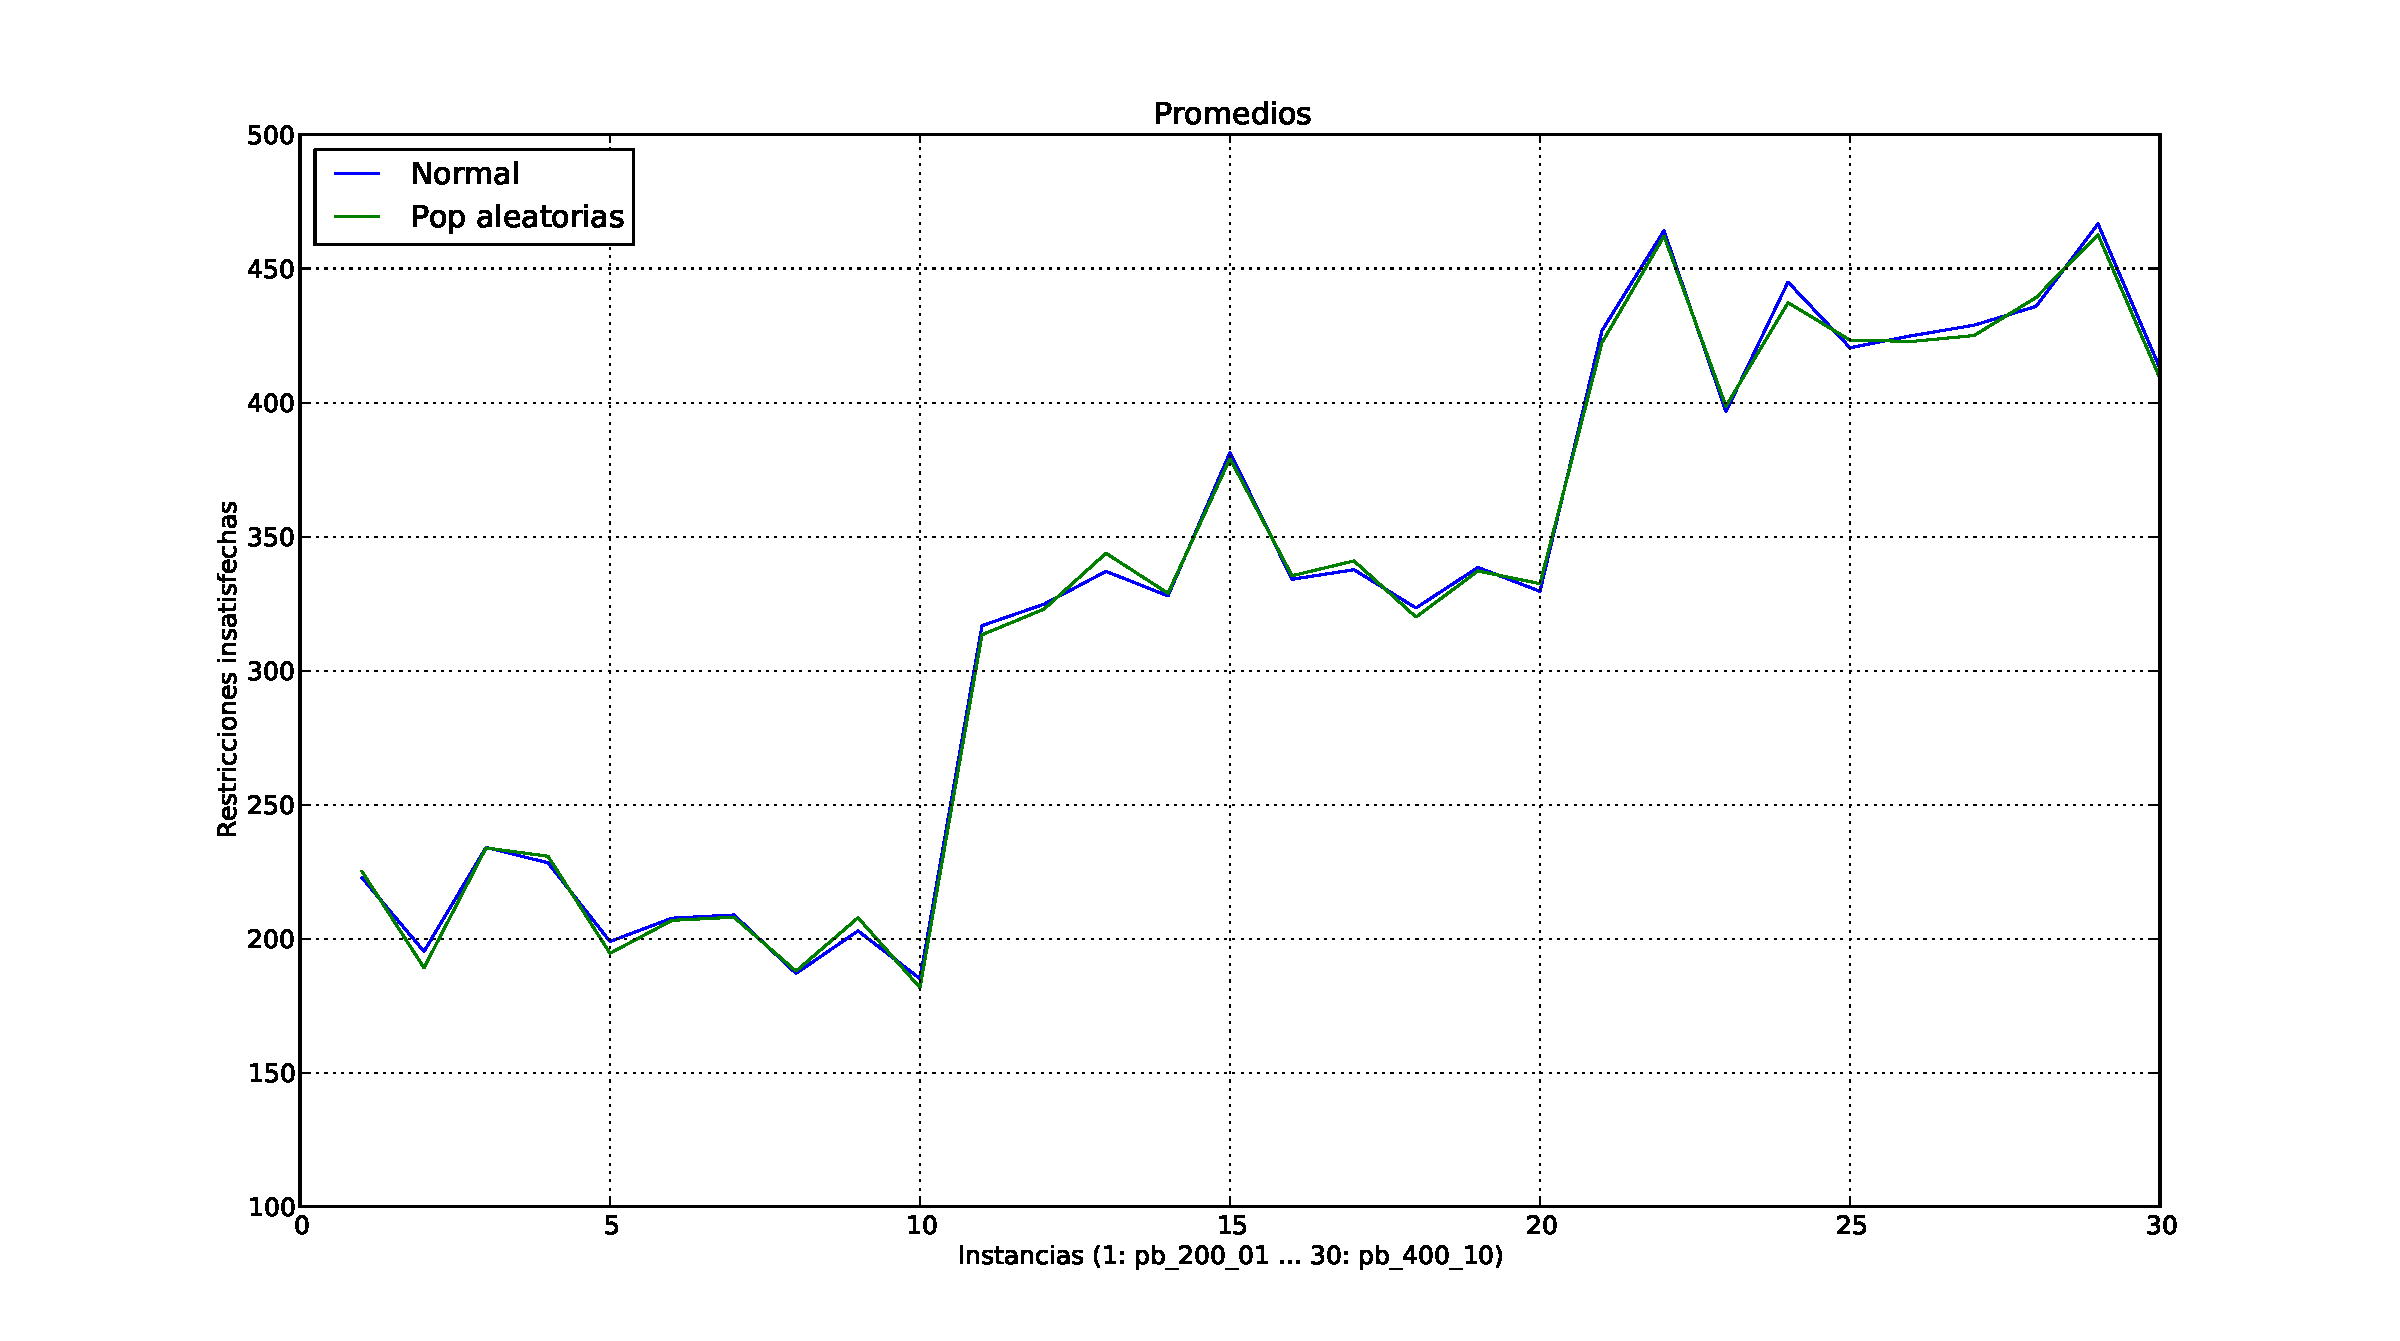
\includegraphics[width=0.95\textwidth]{img/prom-1.pdf}
\end{center}
\caption{Promedio de valores para cada modificación}
\label{fig:prom-1}
\end{figure}

\begin{figure}[h!]
\begin{center}
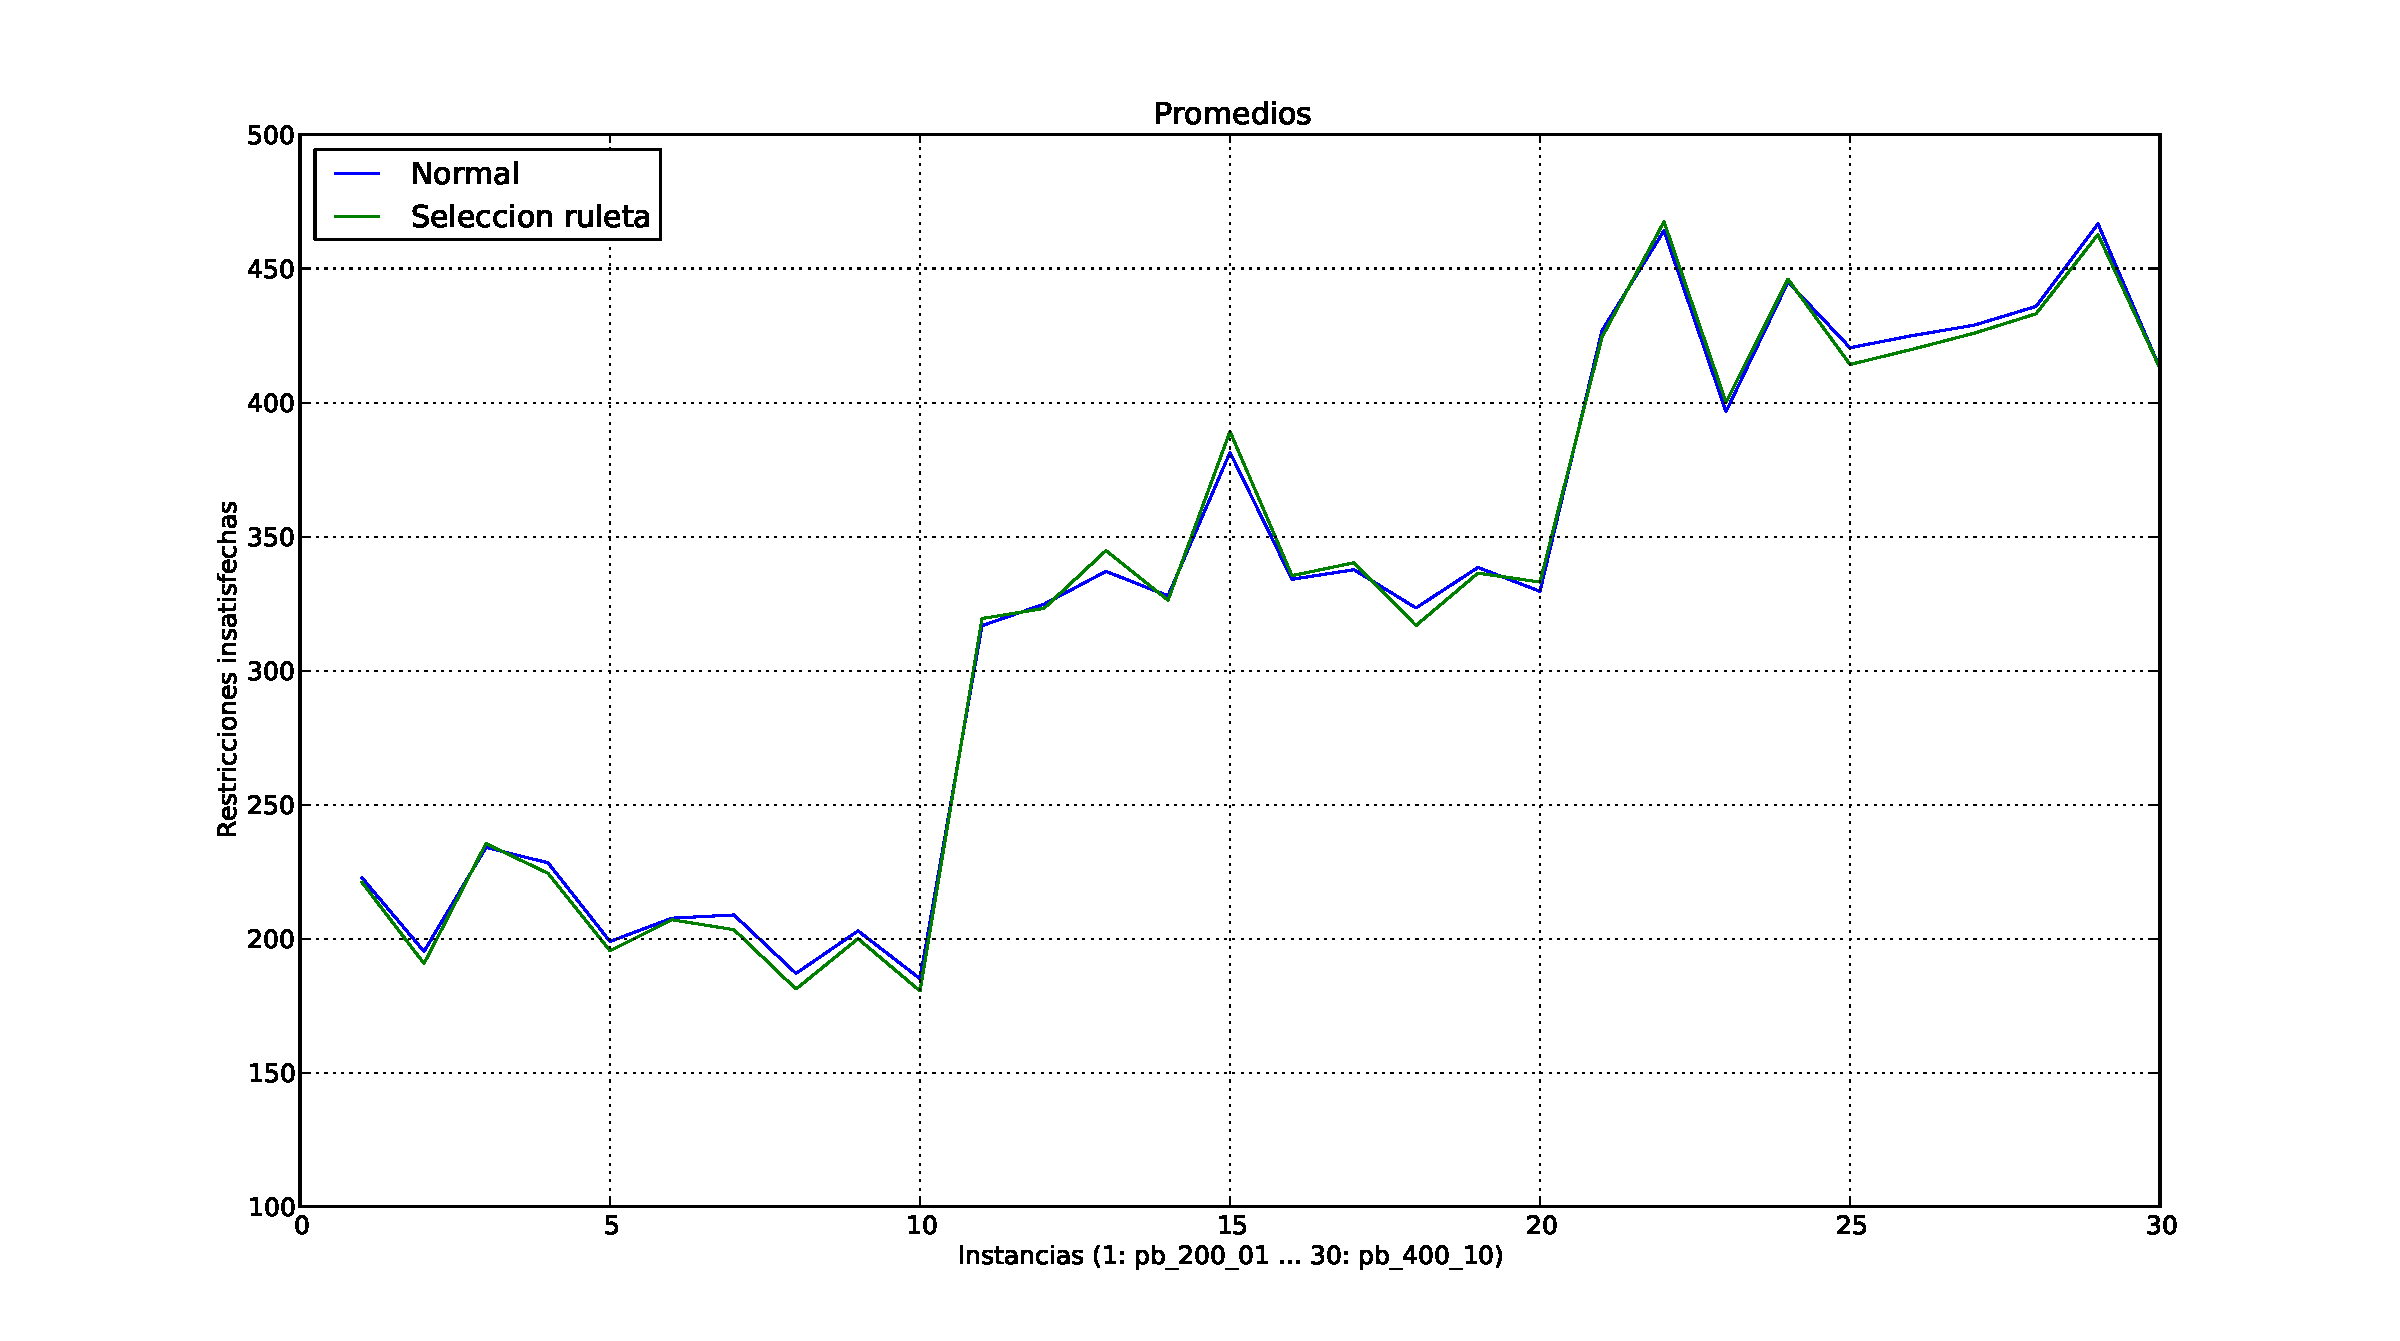
\includegraphics[width=0.95\textwidth]{img/prom-2.pdf}
\end{center}
\caption{Promedio de valores para cada modificación}
\label{fig:prom-2}
\end{figure}

\begin{figure}[h!]
\begin{center}
\includegraphics[width=0.95\textwidth]{img/prom-3.pdf}
\end{center}
\caption{Promedio de valores para cada modificación}
\label{fig:prom-3}
\end{figure}


\begin{figure}[h!]
\begin{center}
\includegraphics[width=0.95\textwidth]{img/prom-4.pdf}
\end{center}
\caption{Promedio de valores para cada modificación}
\label{fig:prom-4}
\end{figure}

\newpage

\subsection{Desviación estándar}

\begin{figure}[h!]
\begin{center}
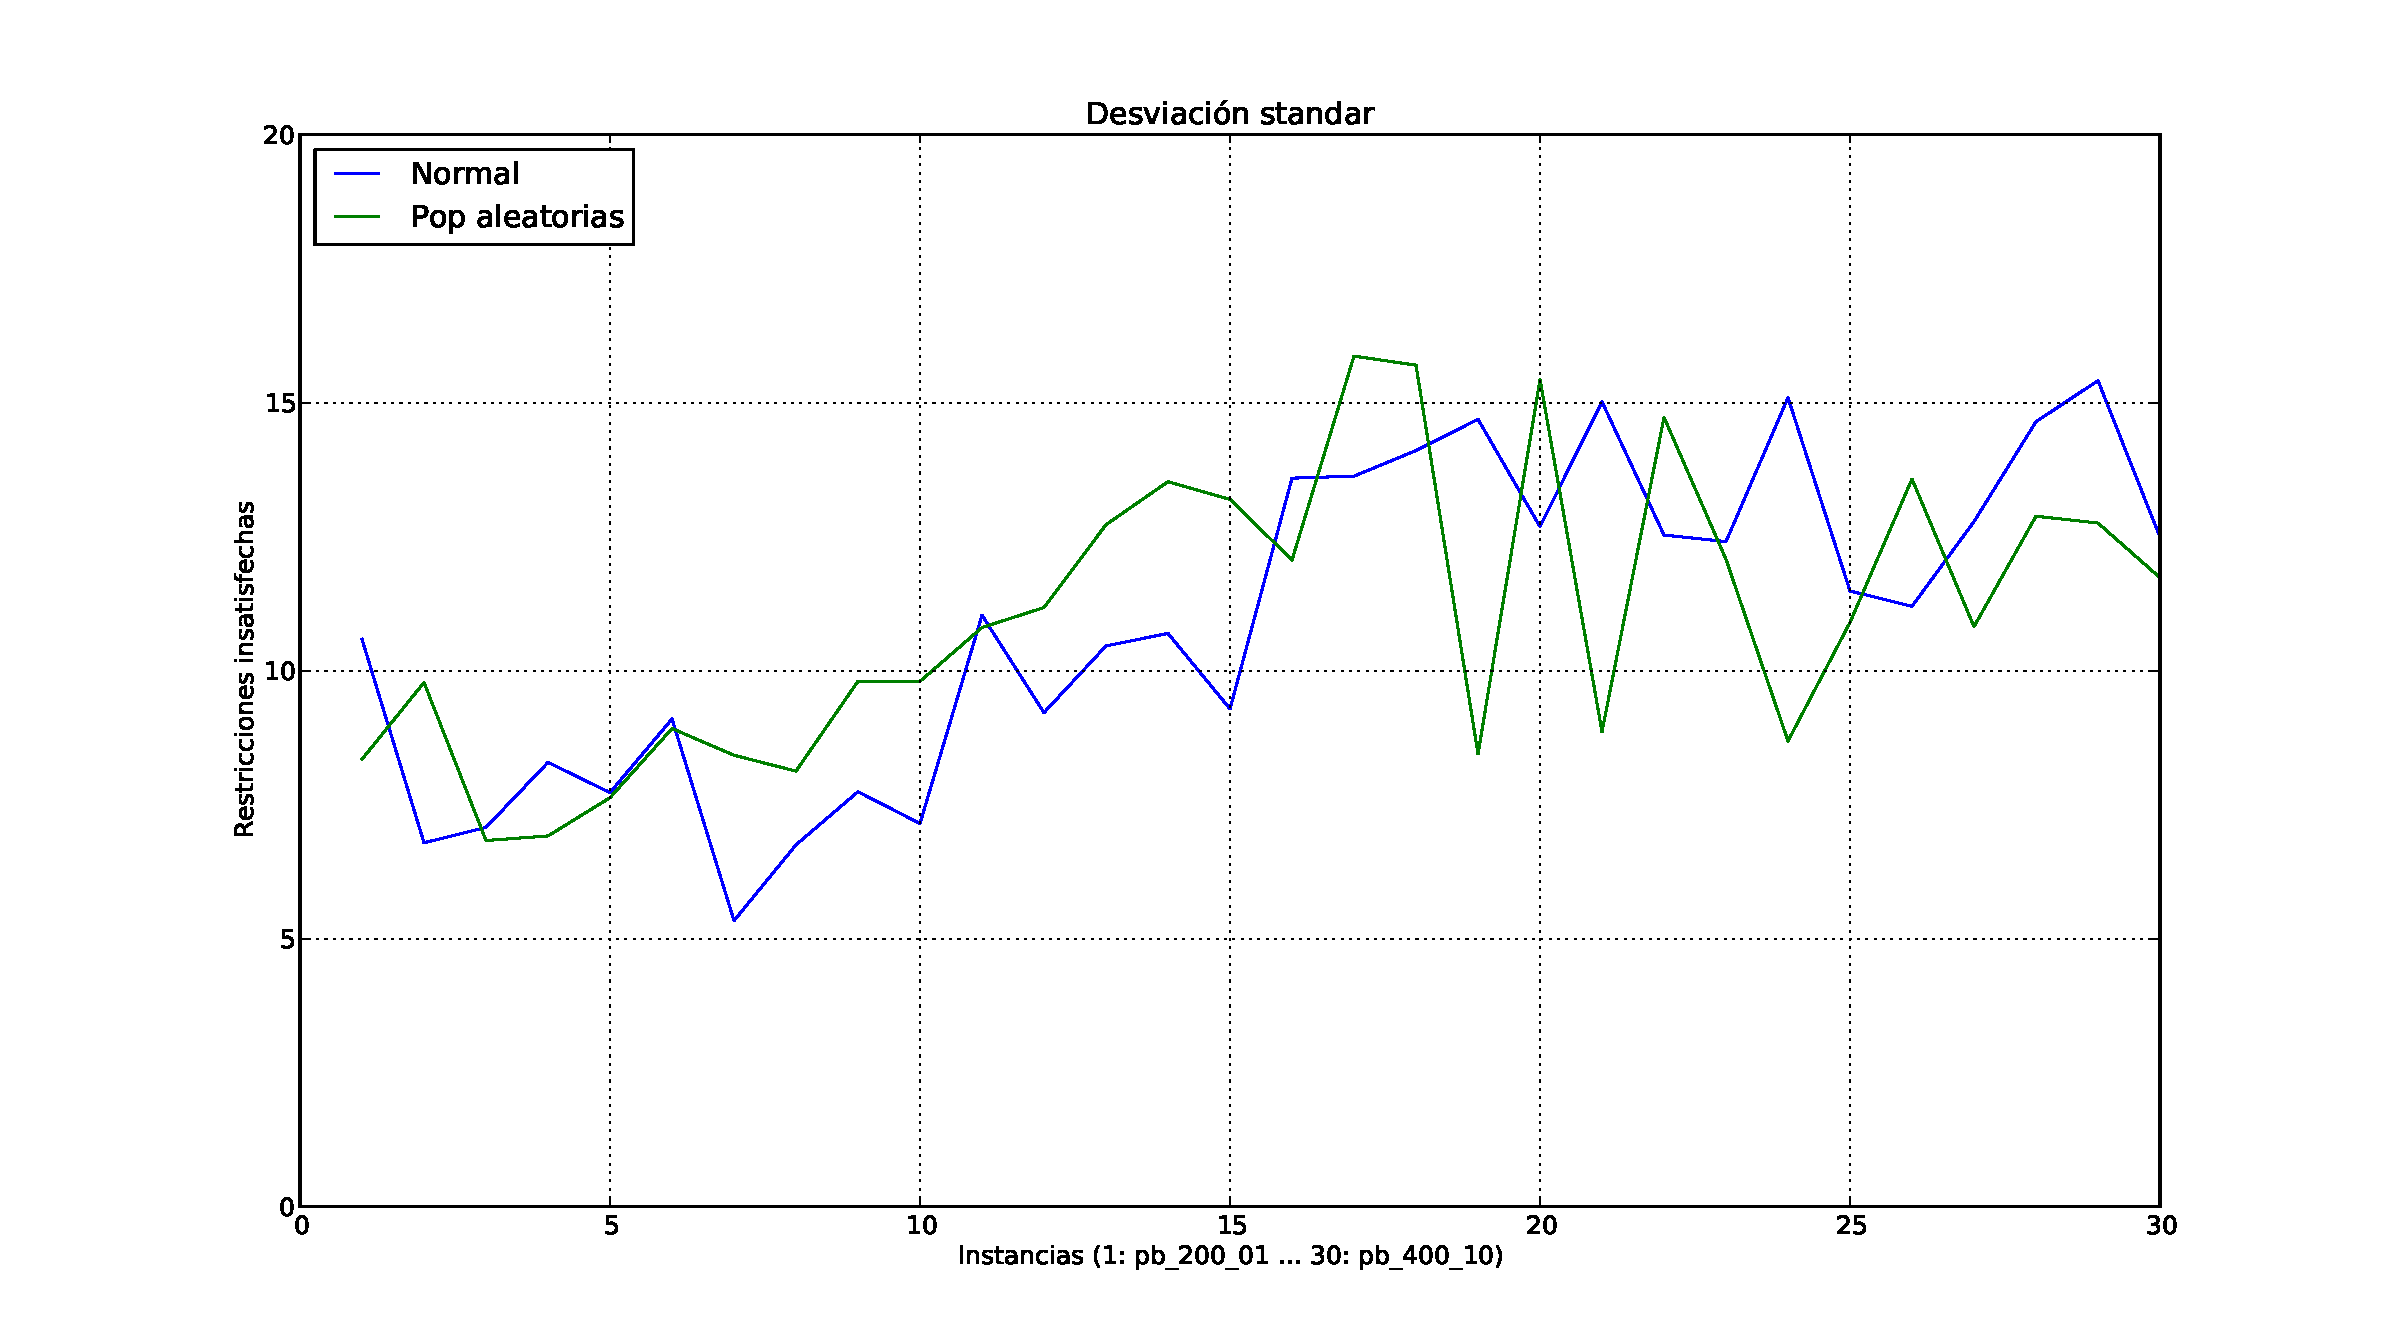
\includegraphics[width=0.95\textwidth]{img/s-1.pdf}
\end{center}
\caption{Desviación estándar para cada modificación.}
\label{fig:s-1}
\end{figure}

\begin{figure}[h!]
\begin{center}
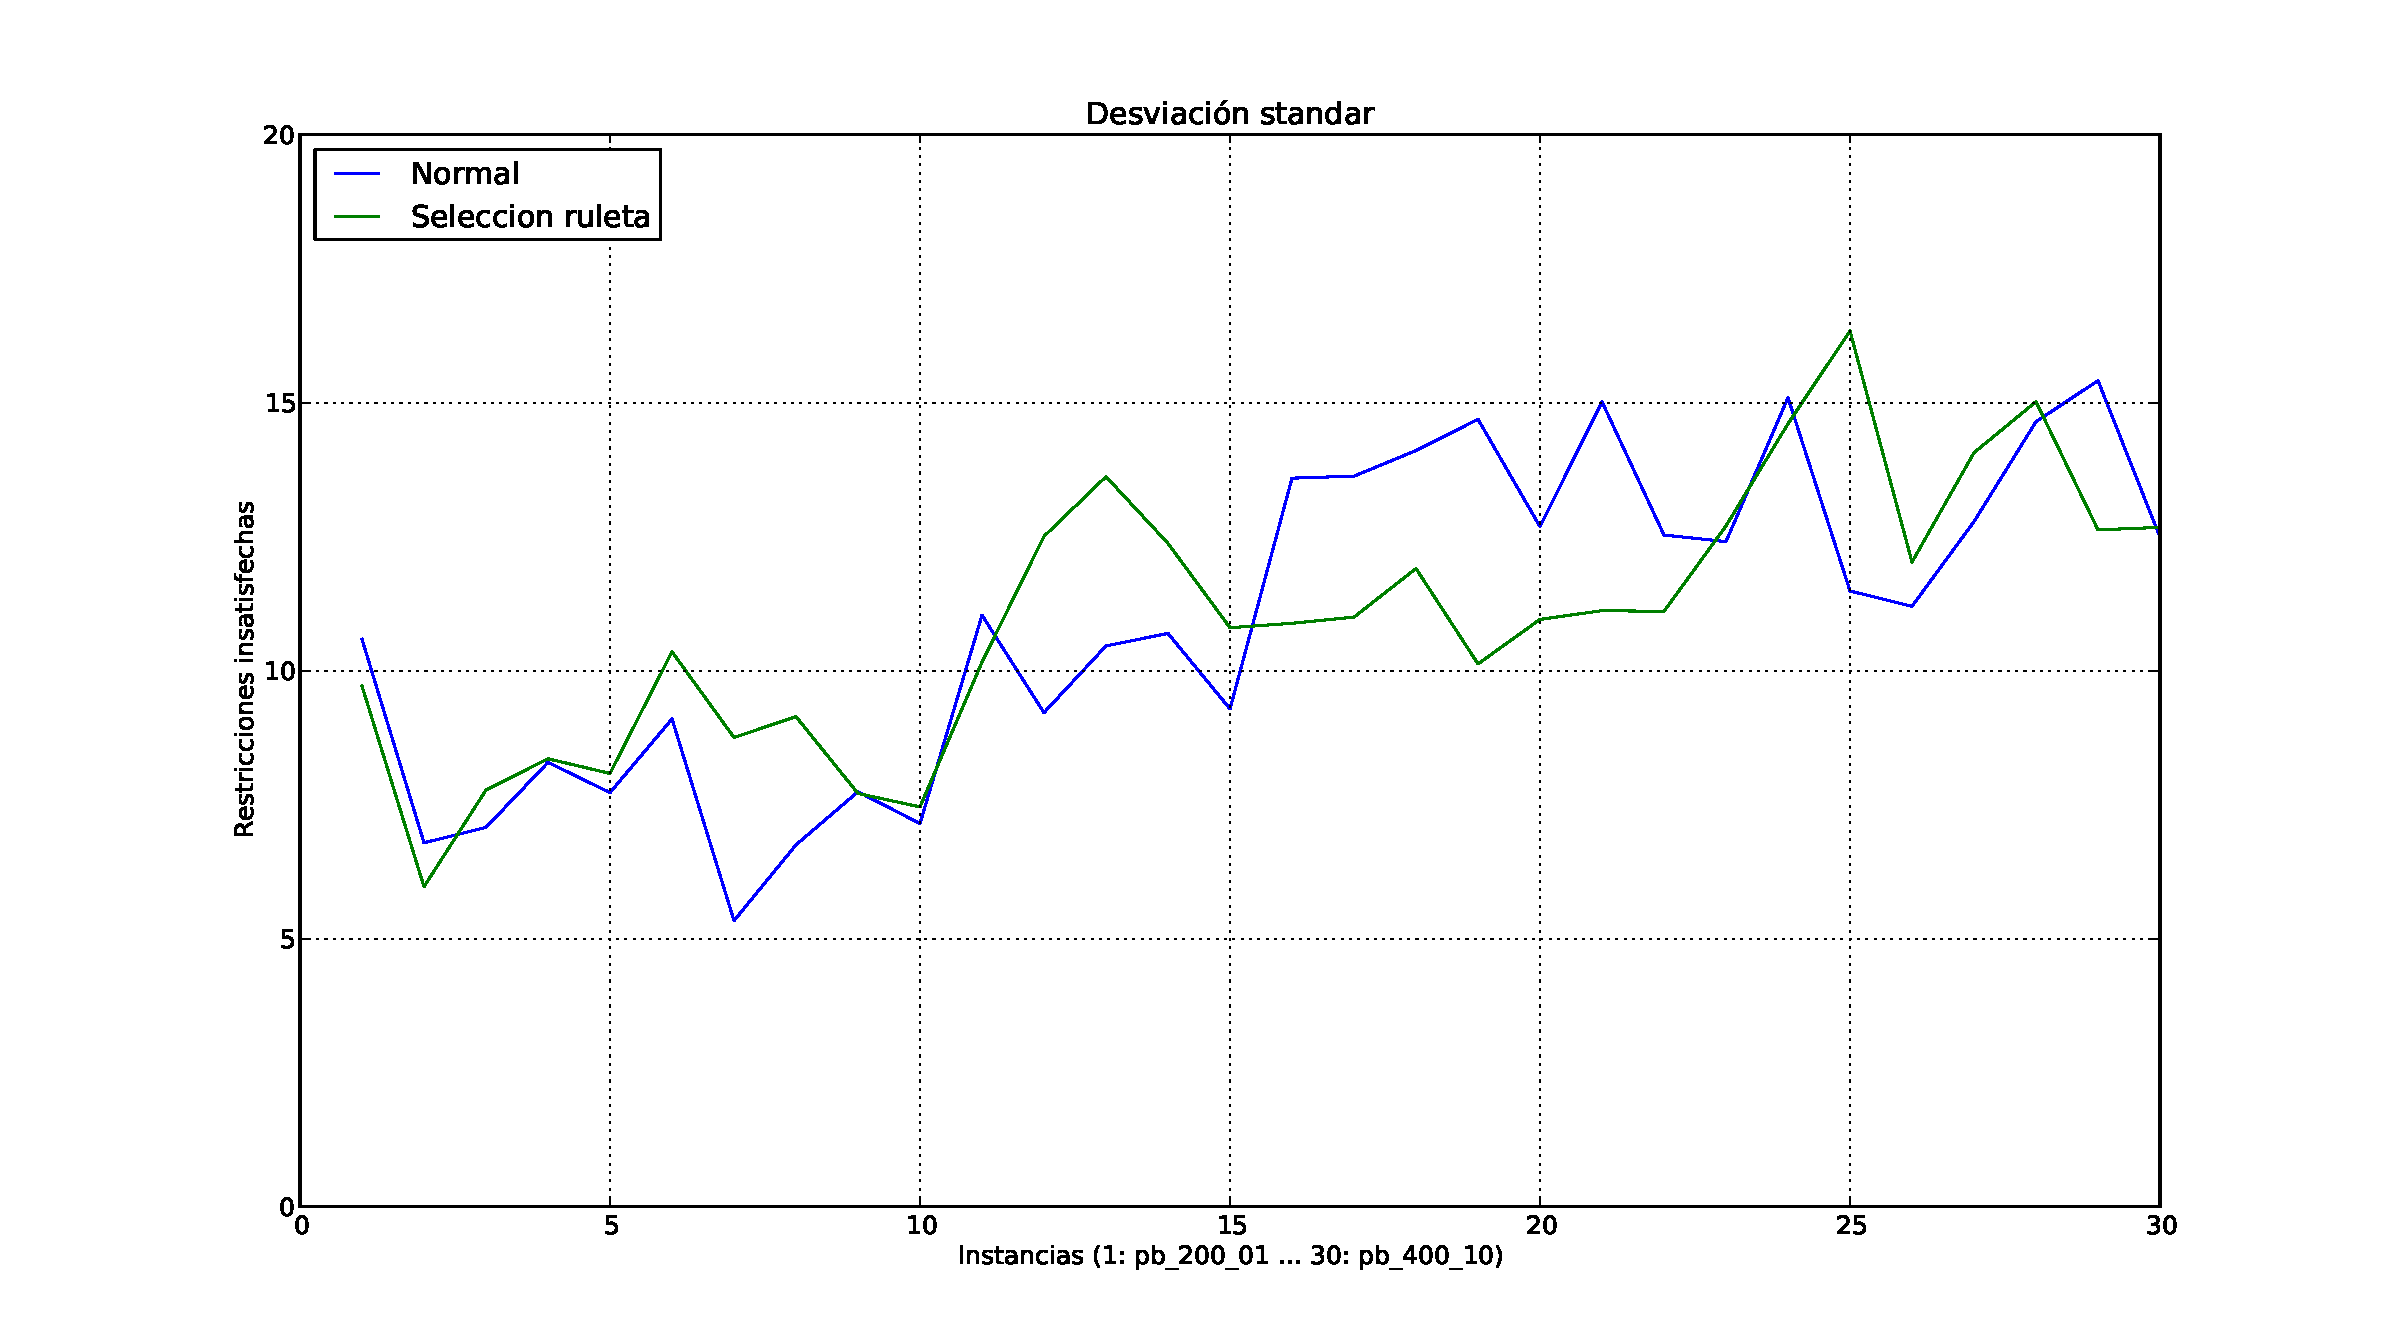
\includegraphics[width=0.95\textwidth]{img/s-2.pdf}
\end{center}
\caption{Desviación estándar para cada modificación.}
\label{fig:s-2}
\end{figure}

\begin{figure}[h!]
\begin{center}
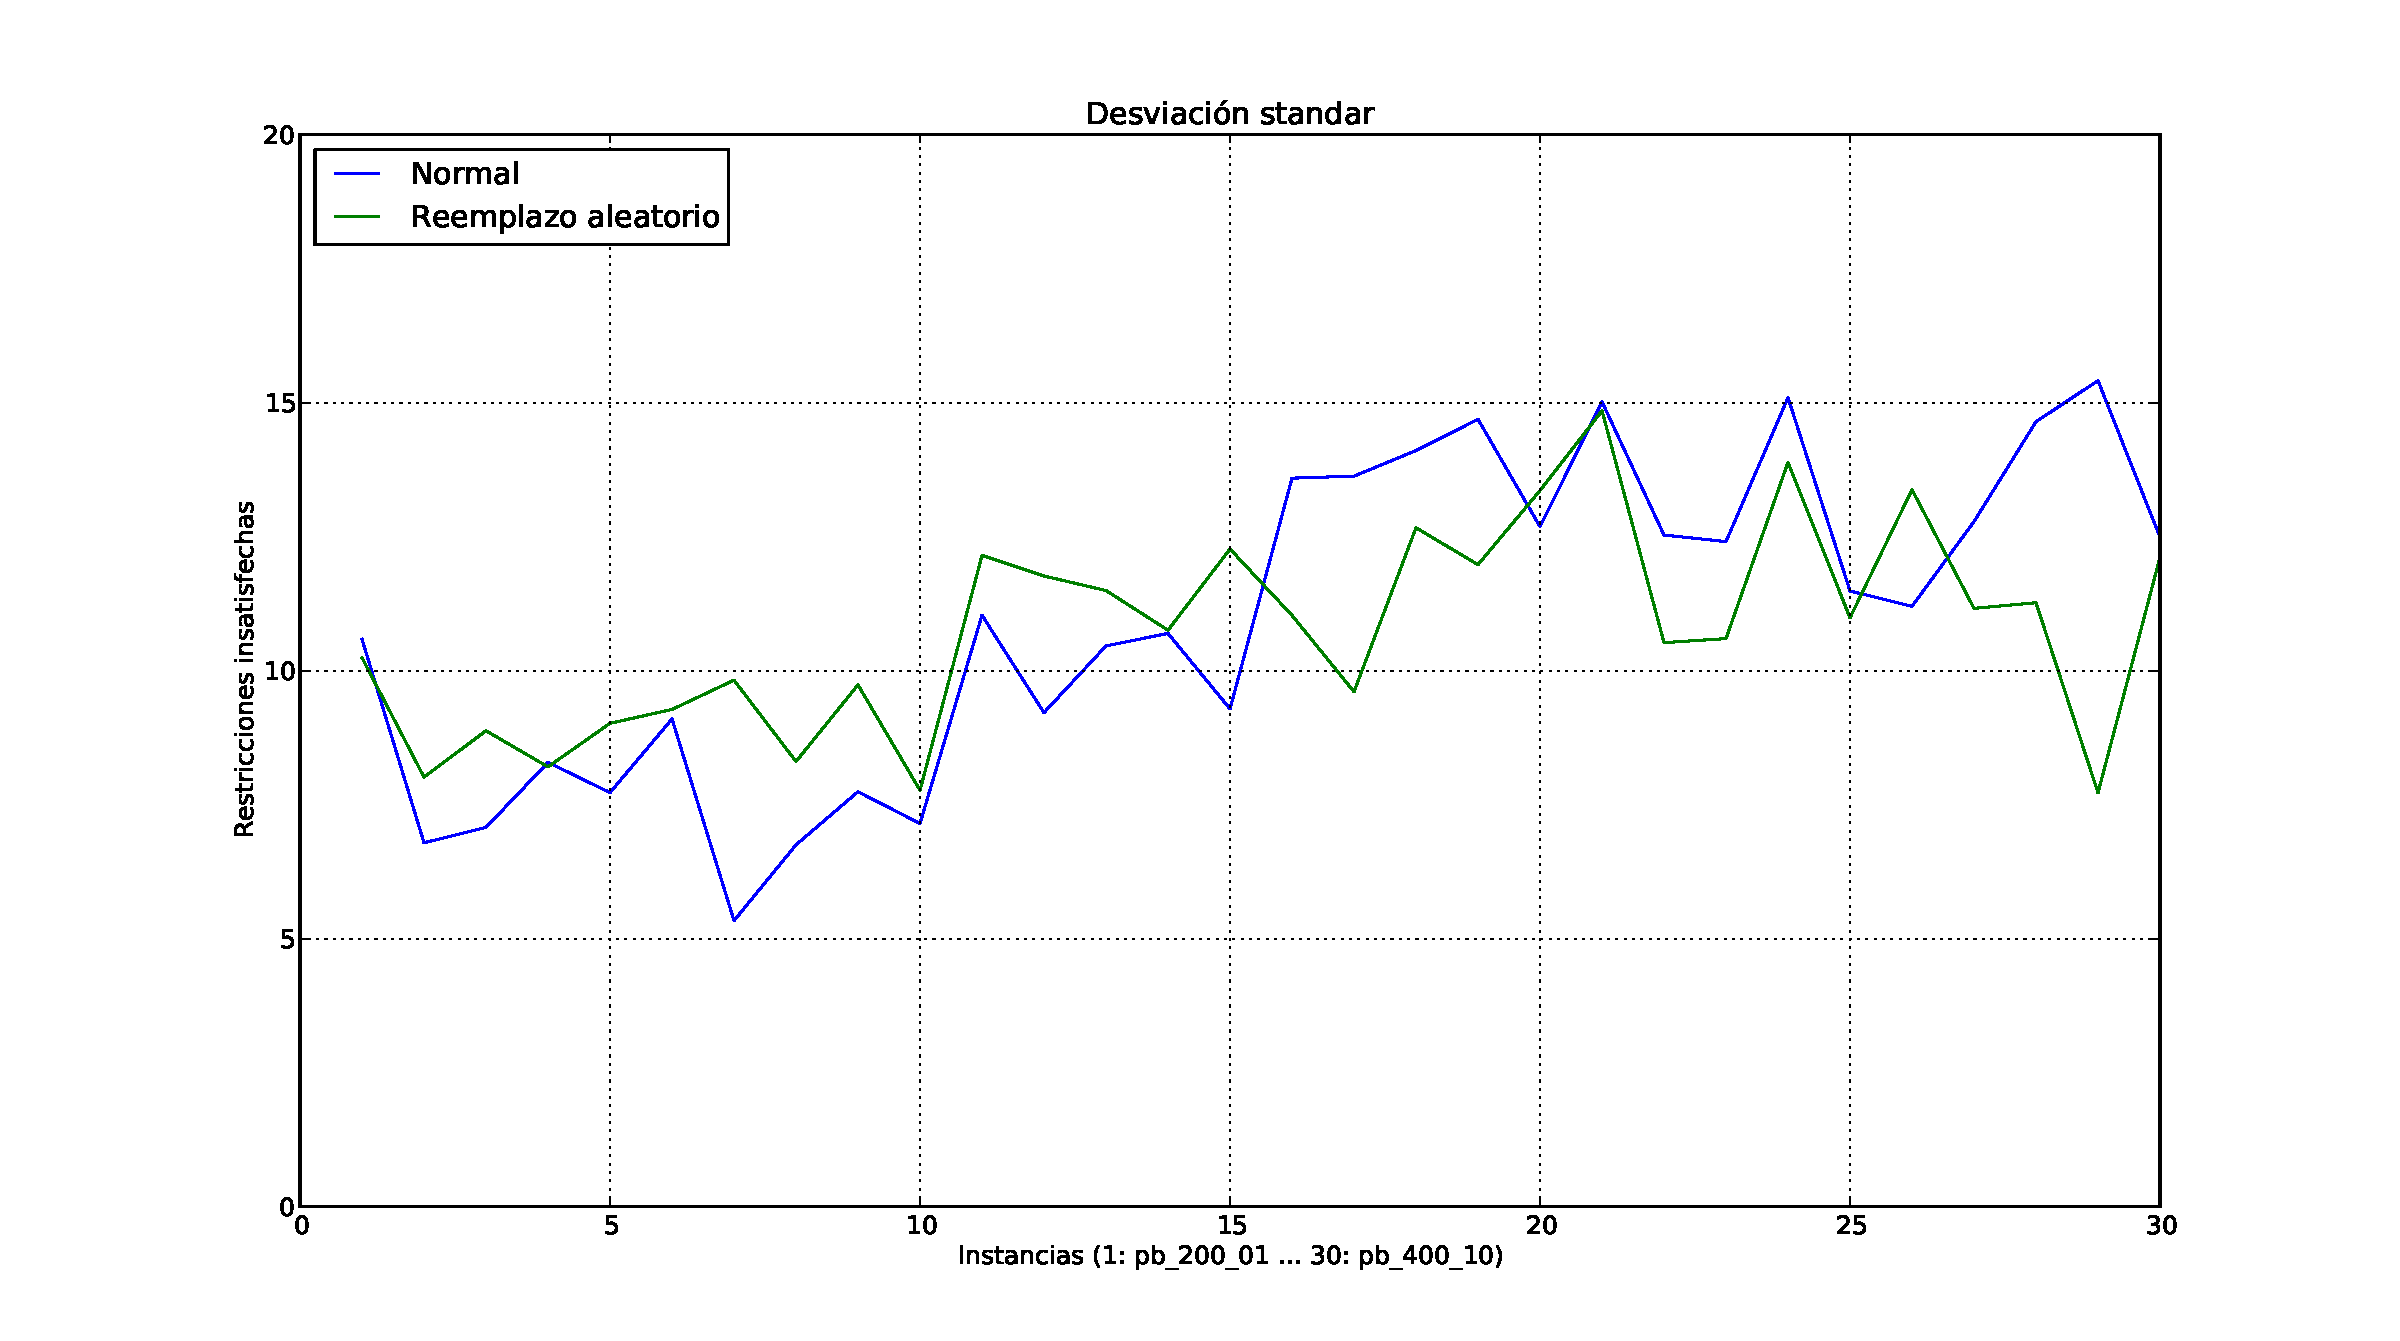
\includegraphics[width=0.95\textwidth]{img/s-3.pdf}
\end{center}
\caption{Desviación estándar para cada modificación.}
\label{fig:s-3}
\end{figure}

\begin{figure}[h!]
\begin{center}
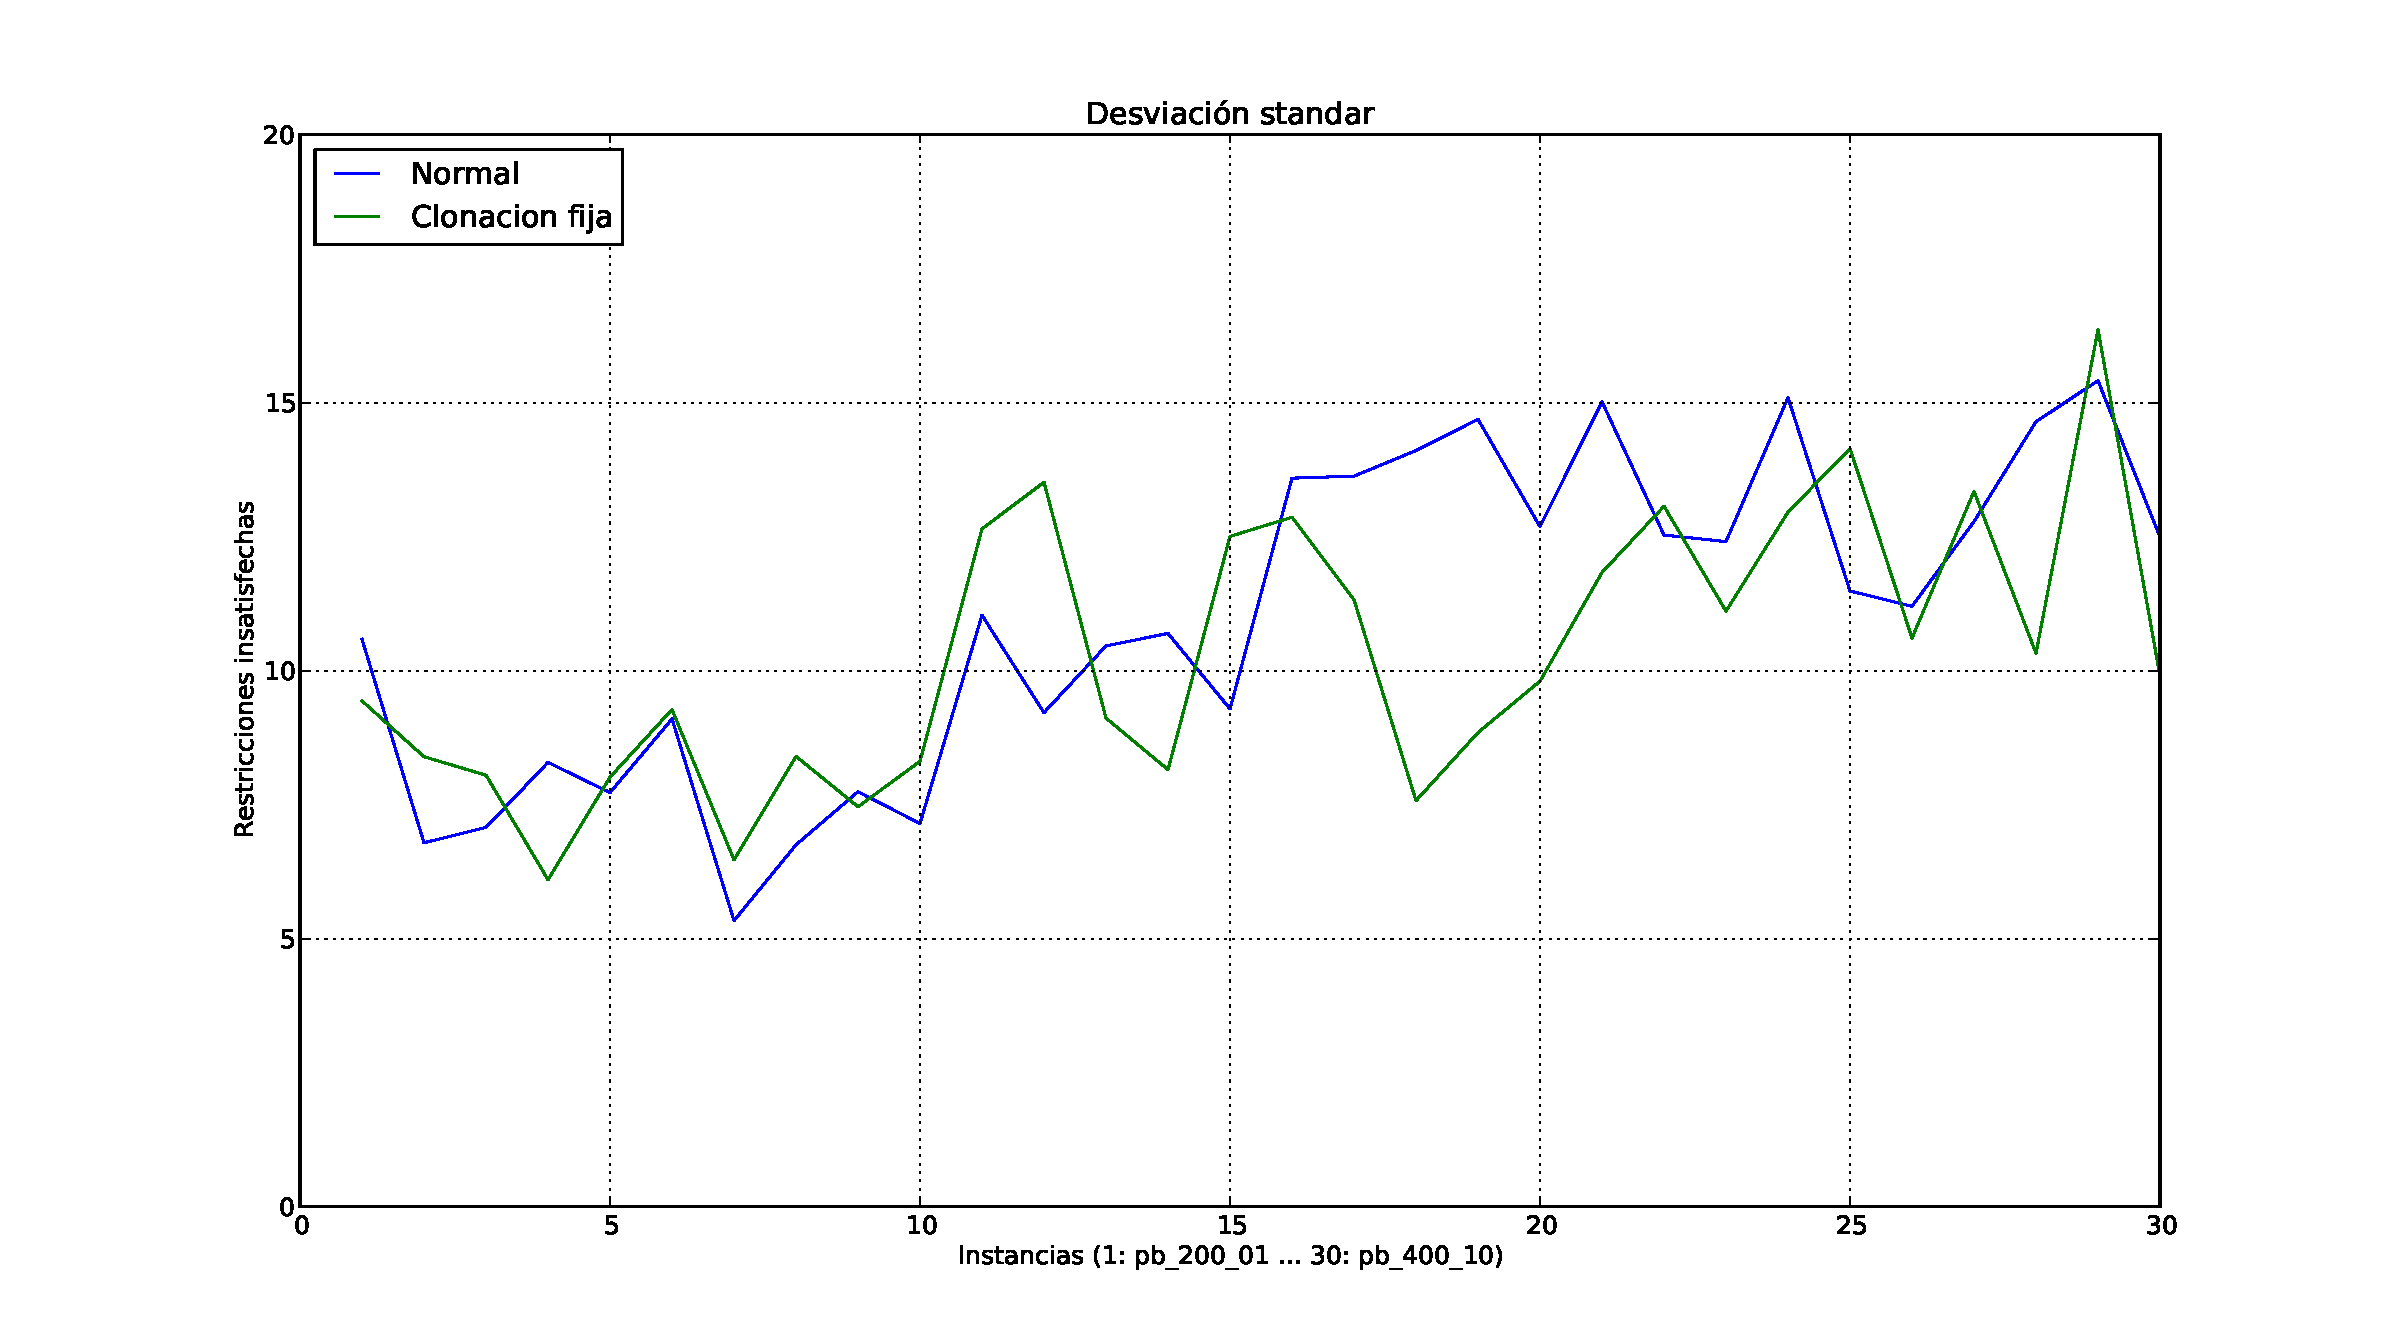
\includegraphics[width=0.95\textwidth]{img/s-4.pdf}
\end{center}
\caption{Desviación estándar para cada modificación.}
\label{fig:s-4}
\end{figure}

\newpage

\subsection{Valores máximos}

\begin{figure}[h!]
\begin{center}
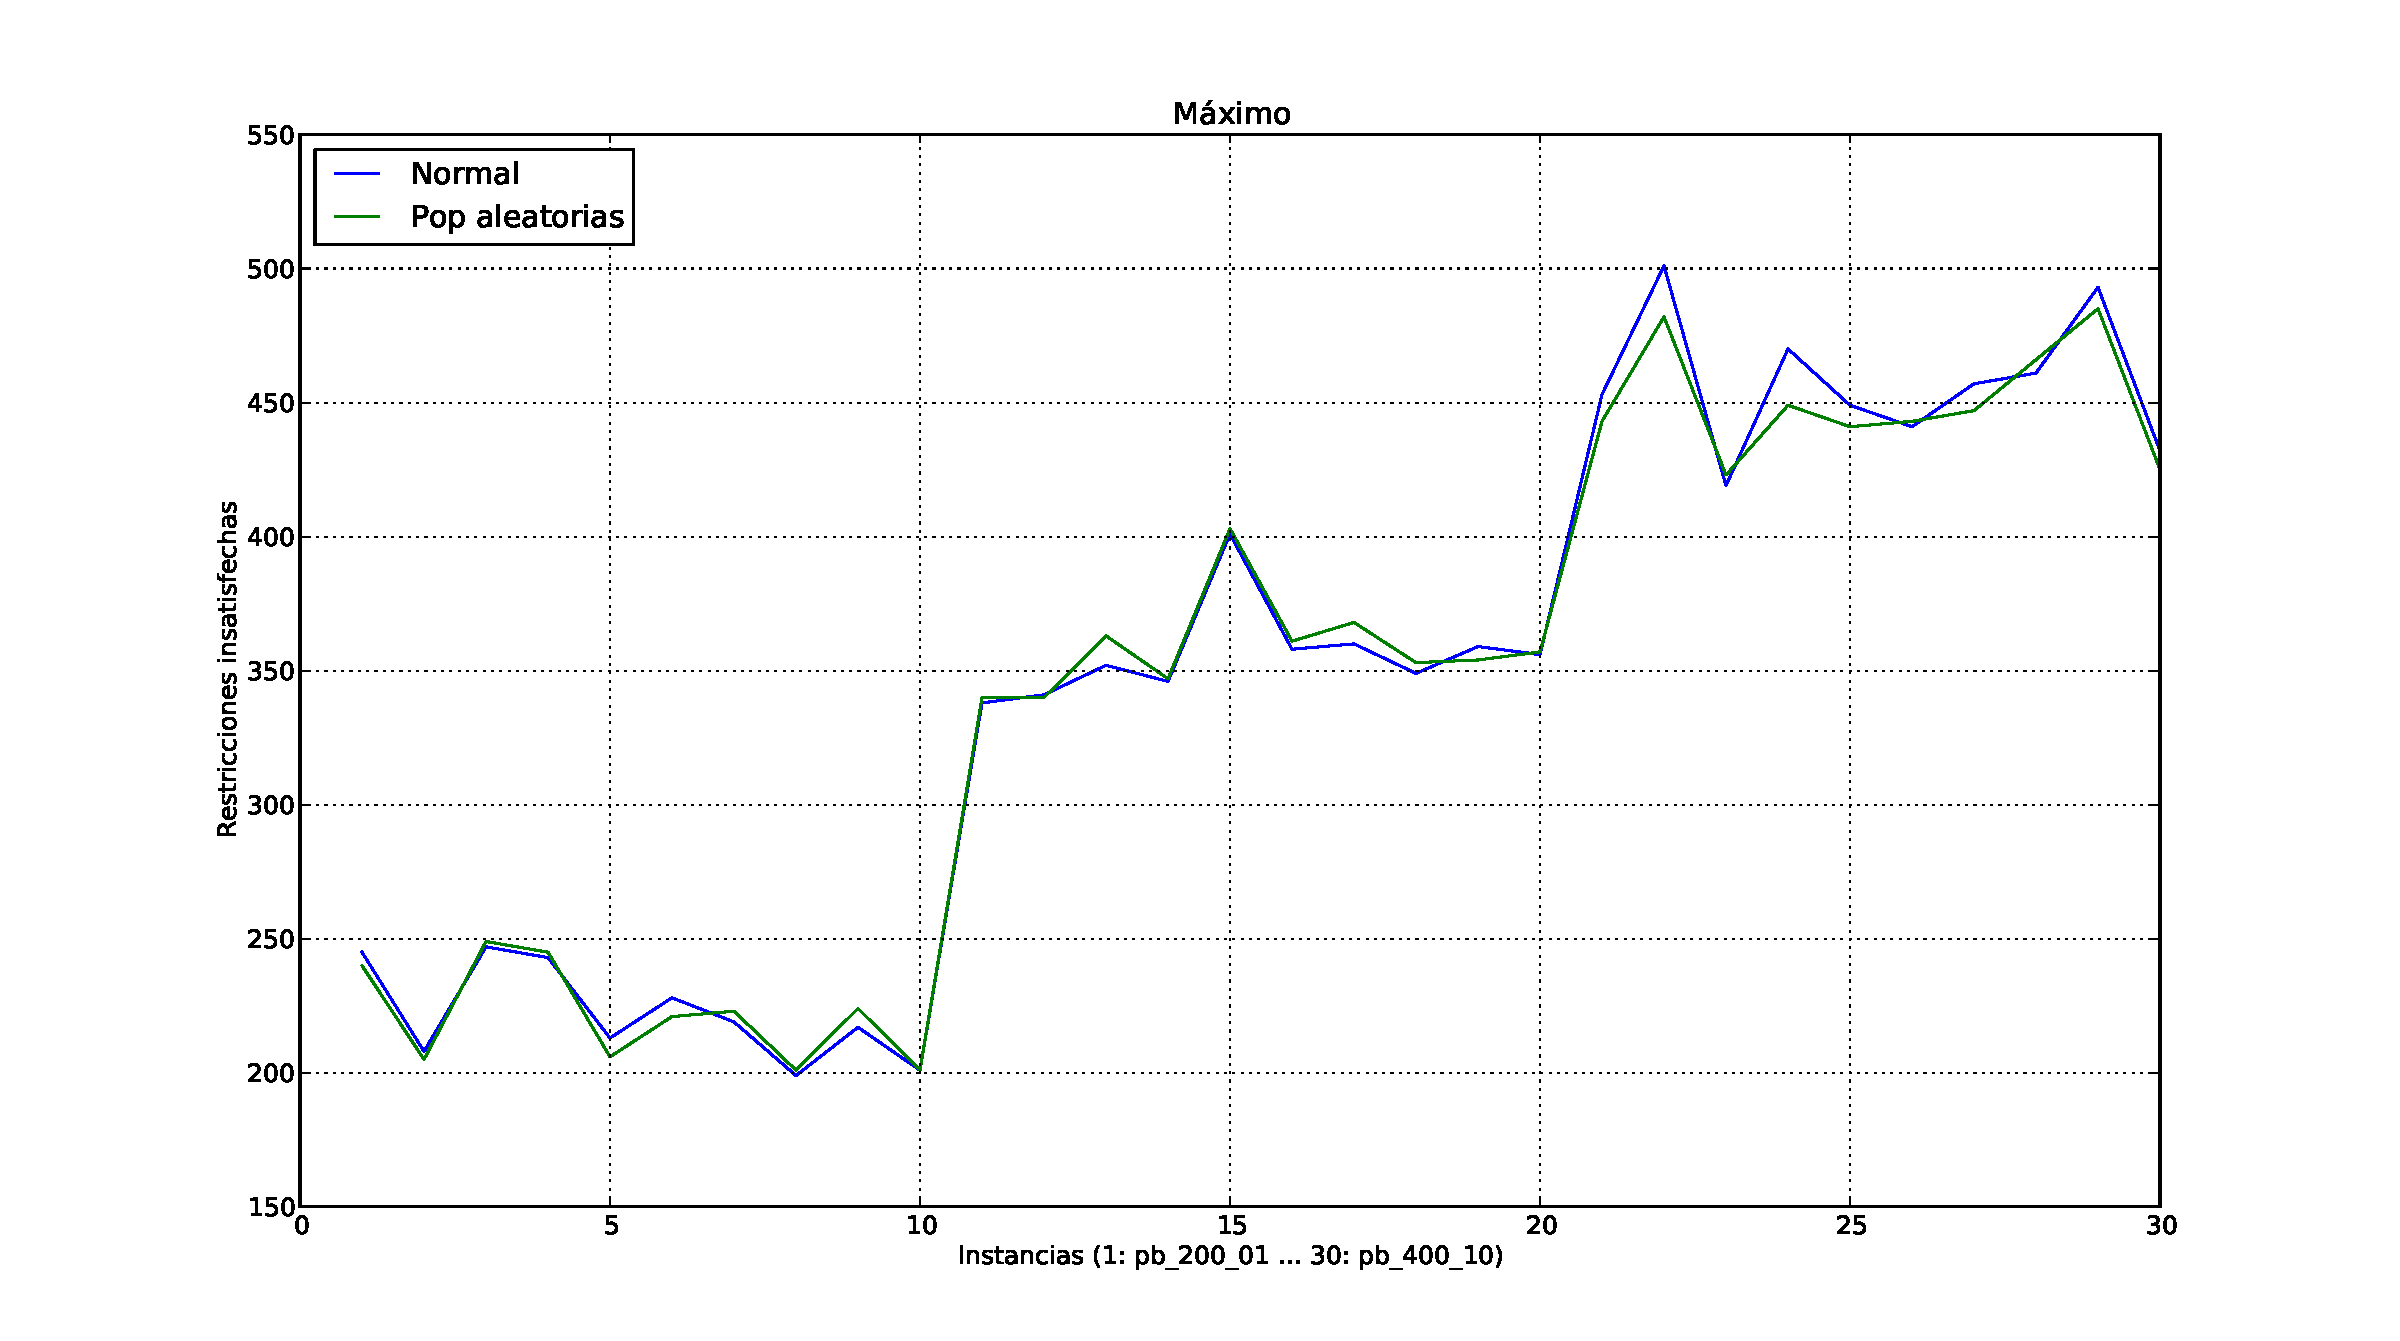
\includegraphics[width=0.95\textwidth]{img/max-1.pdf}
\end{center}
\caption{Valores máximos para cada modificación}
\label{fig:max-1}
\end{figure}

\begin{figure}[h!]
\begin{center}
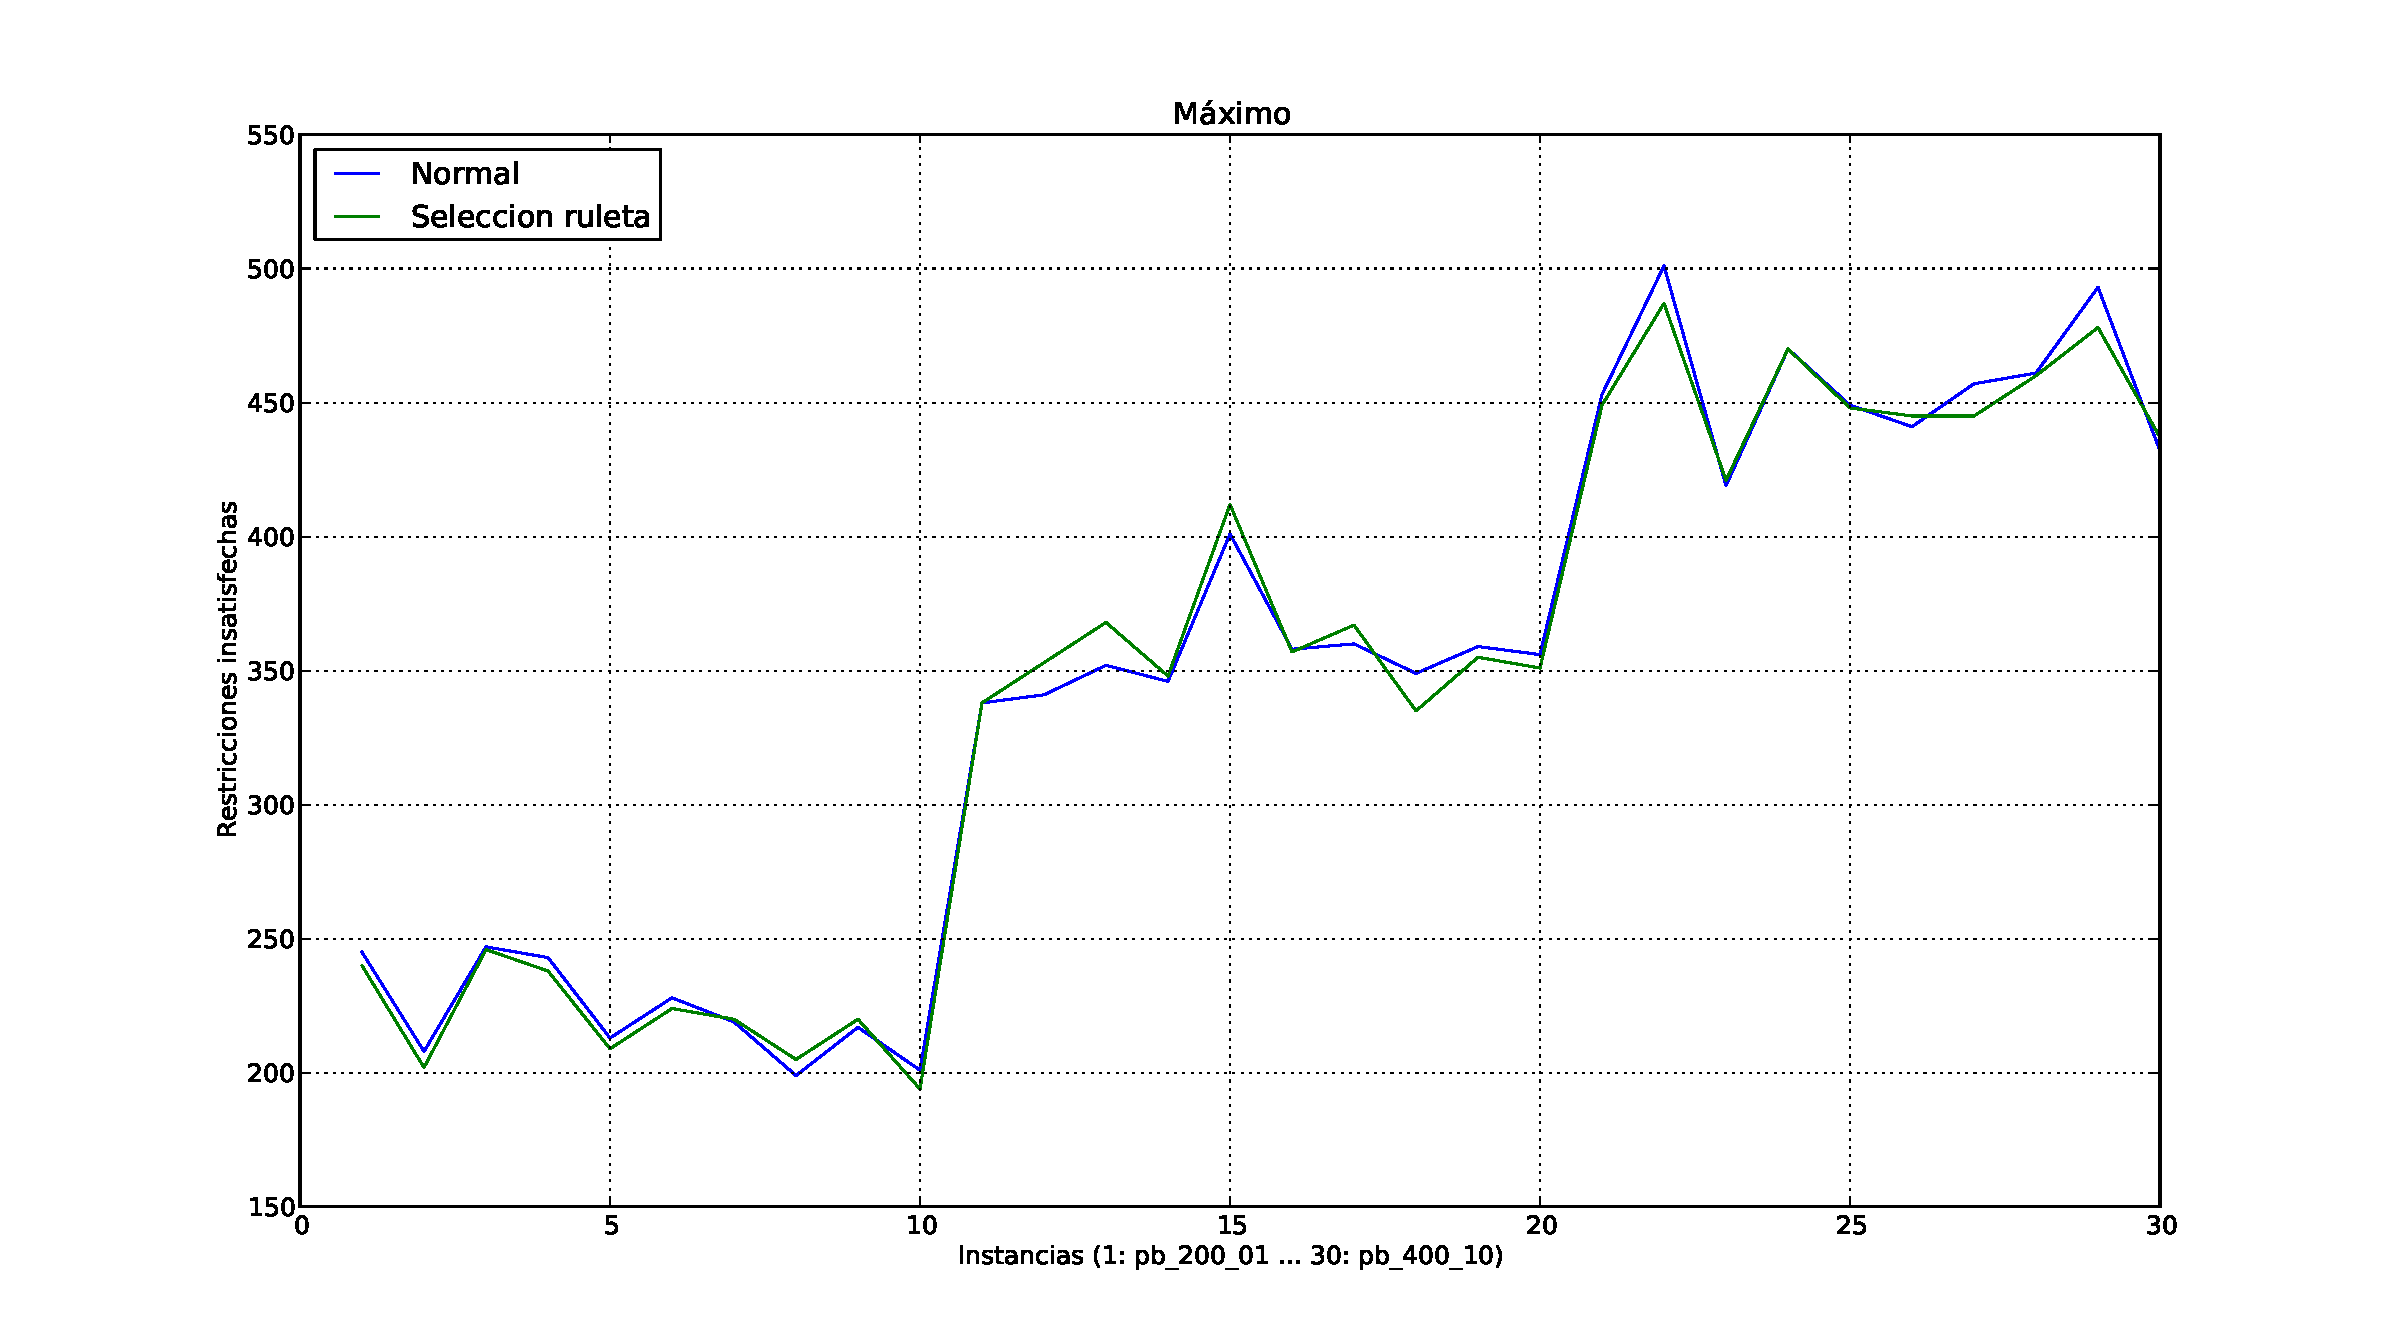
\includegraphics[width=0.95\textwidth]{img/max-2.pdf}
\end{center}
\caption{Valores máximos para cada modificación}
\label{fig:max-2}
\end{figure}

\begin{figure}[h!]
\begin{center}
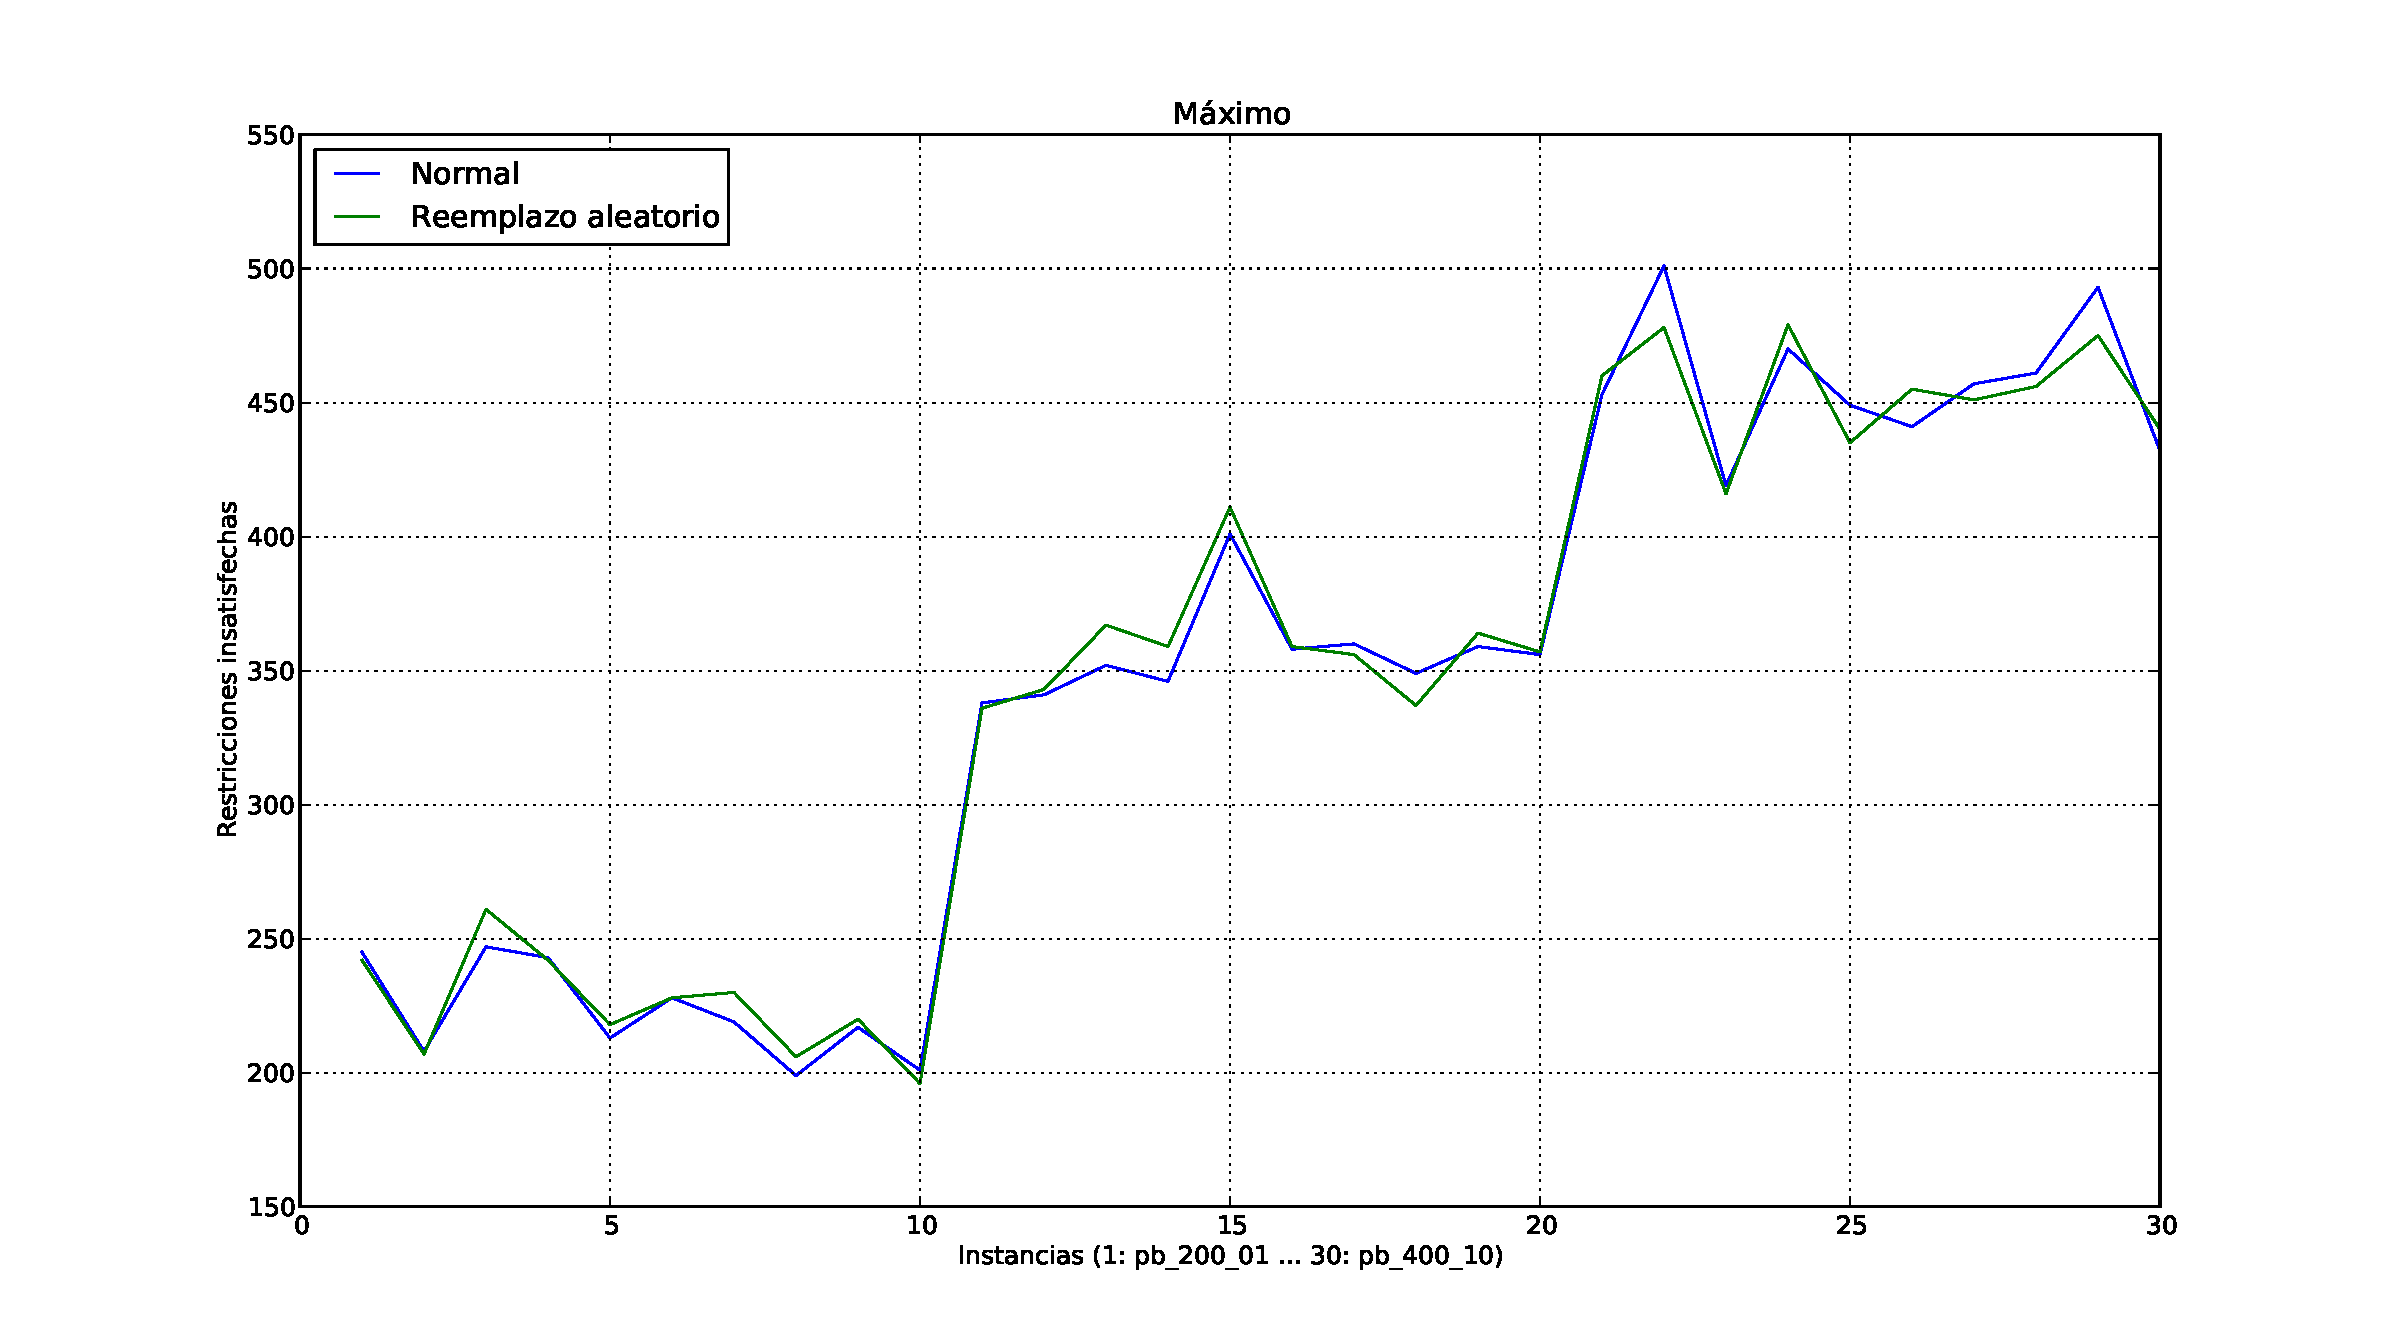
\includegraphics[width=0.95\textwidth]{img/max-3.pdf}
\end{center}
\caption{Valores máximos para cada modificación}
\label{fig:max-3}
\end{figure}

\begin{figure}[h!]
\begin{center}
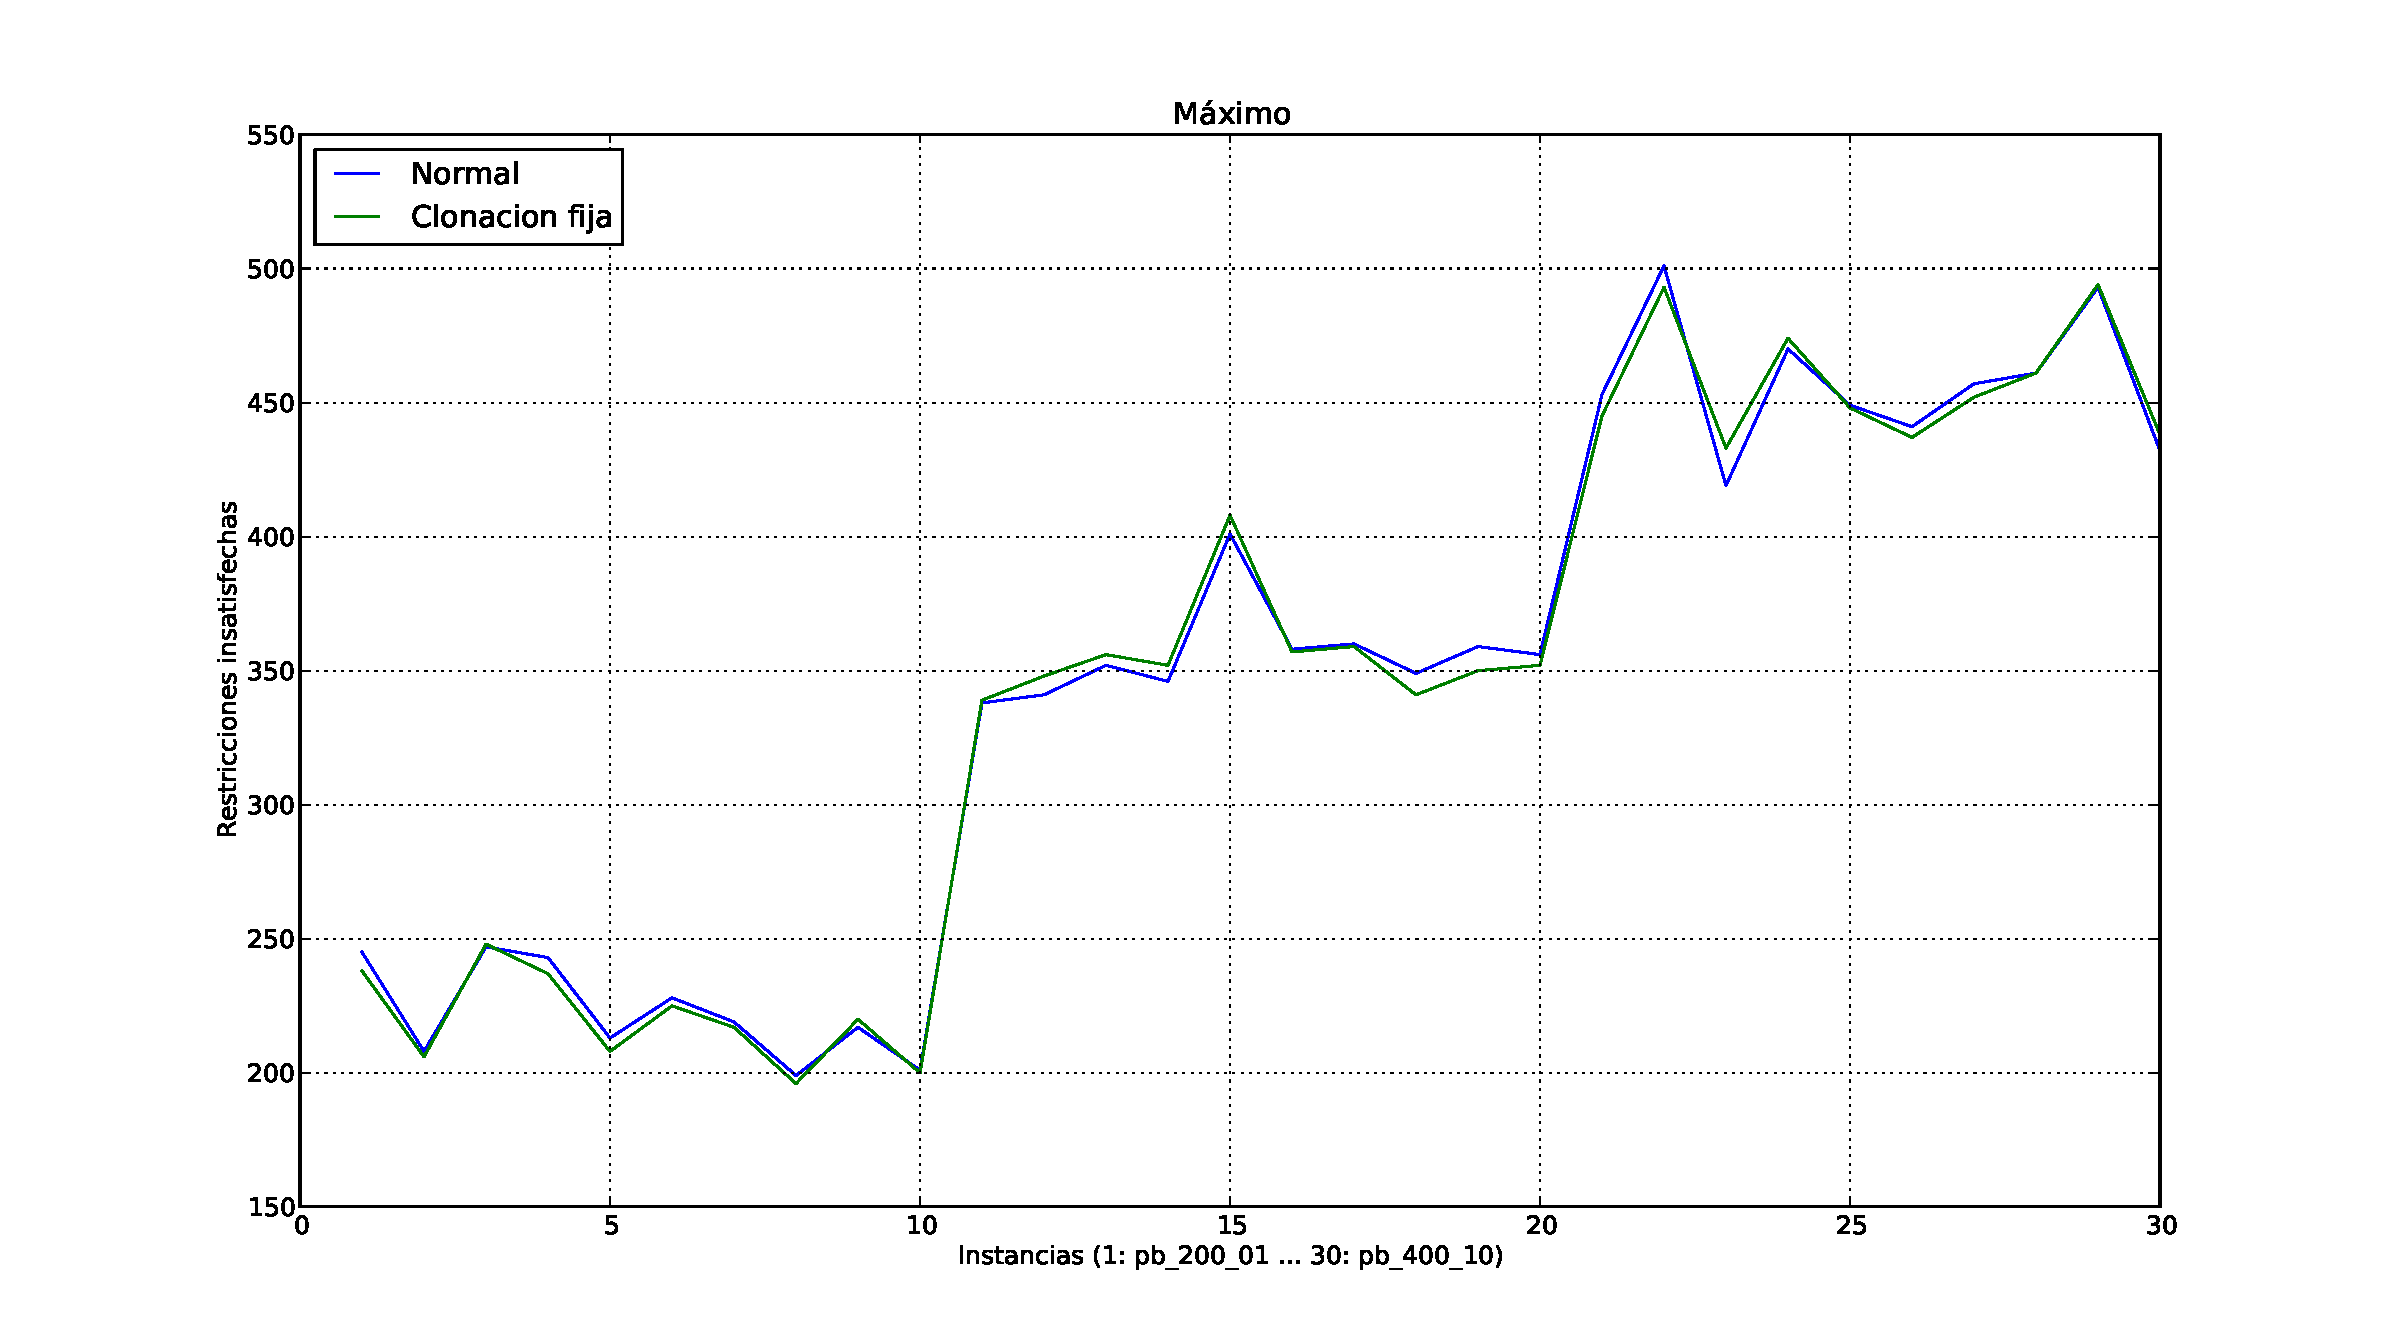
\includegraphics[width=0.95\textwidth]{img/max-4.pdf}
\end{center}
\caption{Valores máximos para cada modificación}
\label{fig:max-4}
\end{figure}


\newpage

\subsection{Valores mínimos}

\begin{figure}[h!]
\begin{center}
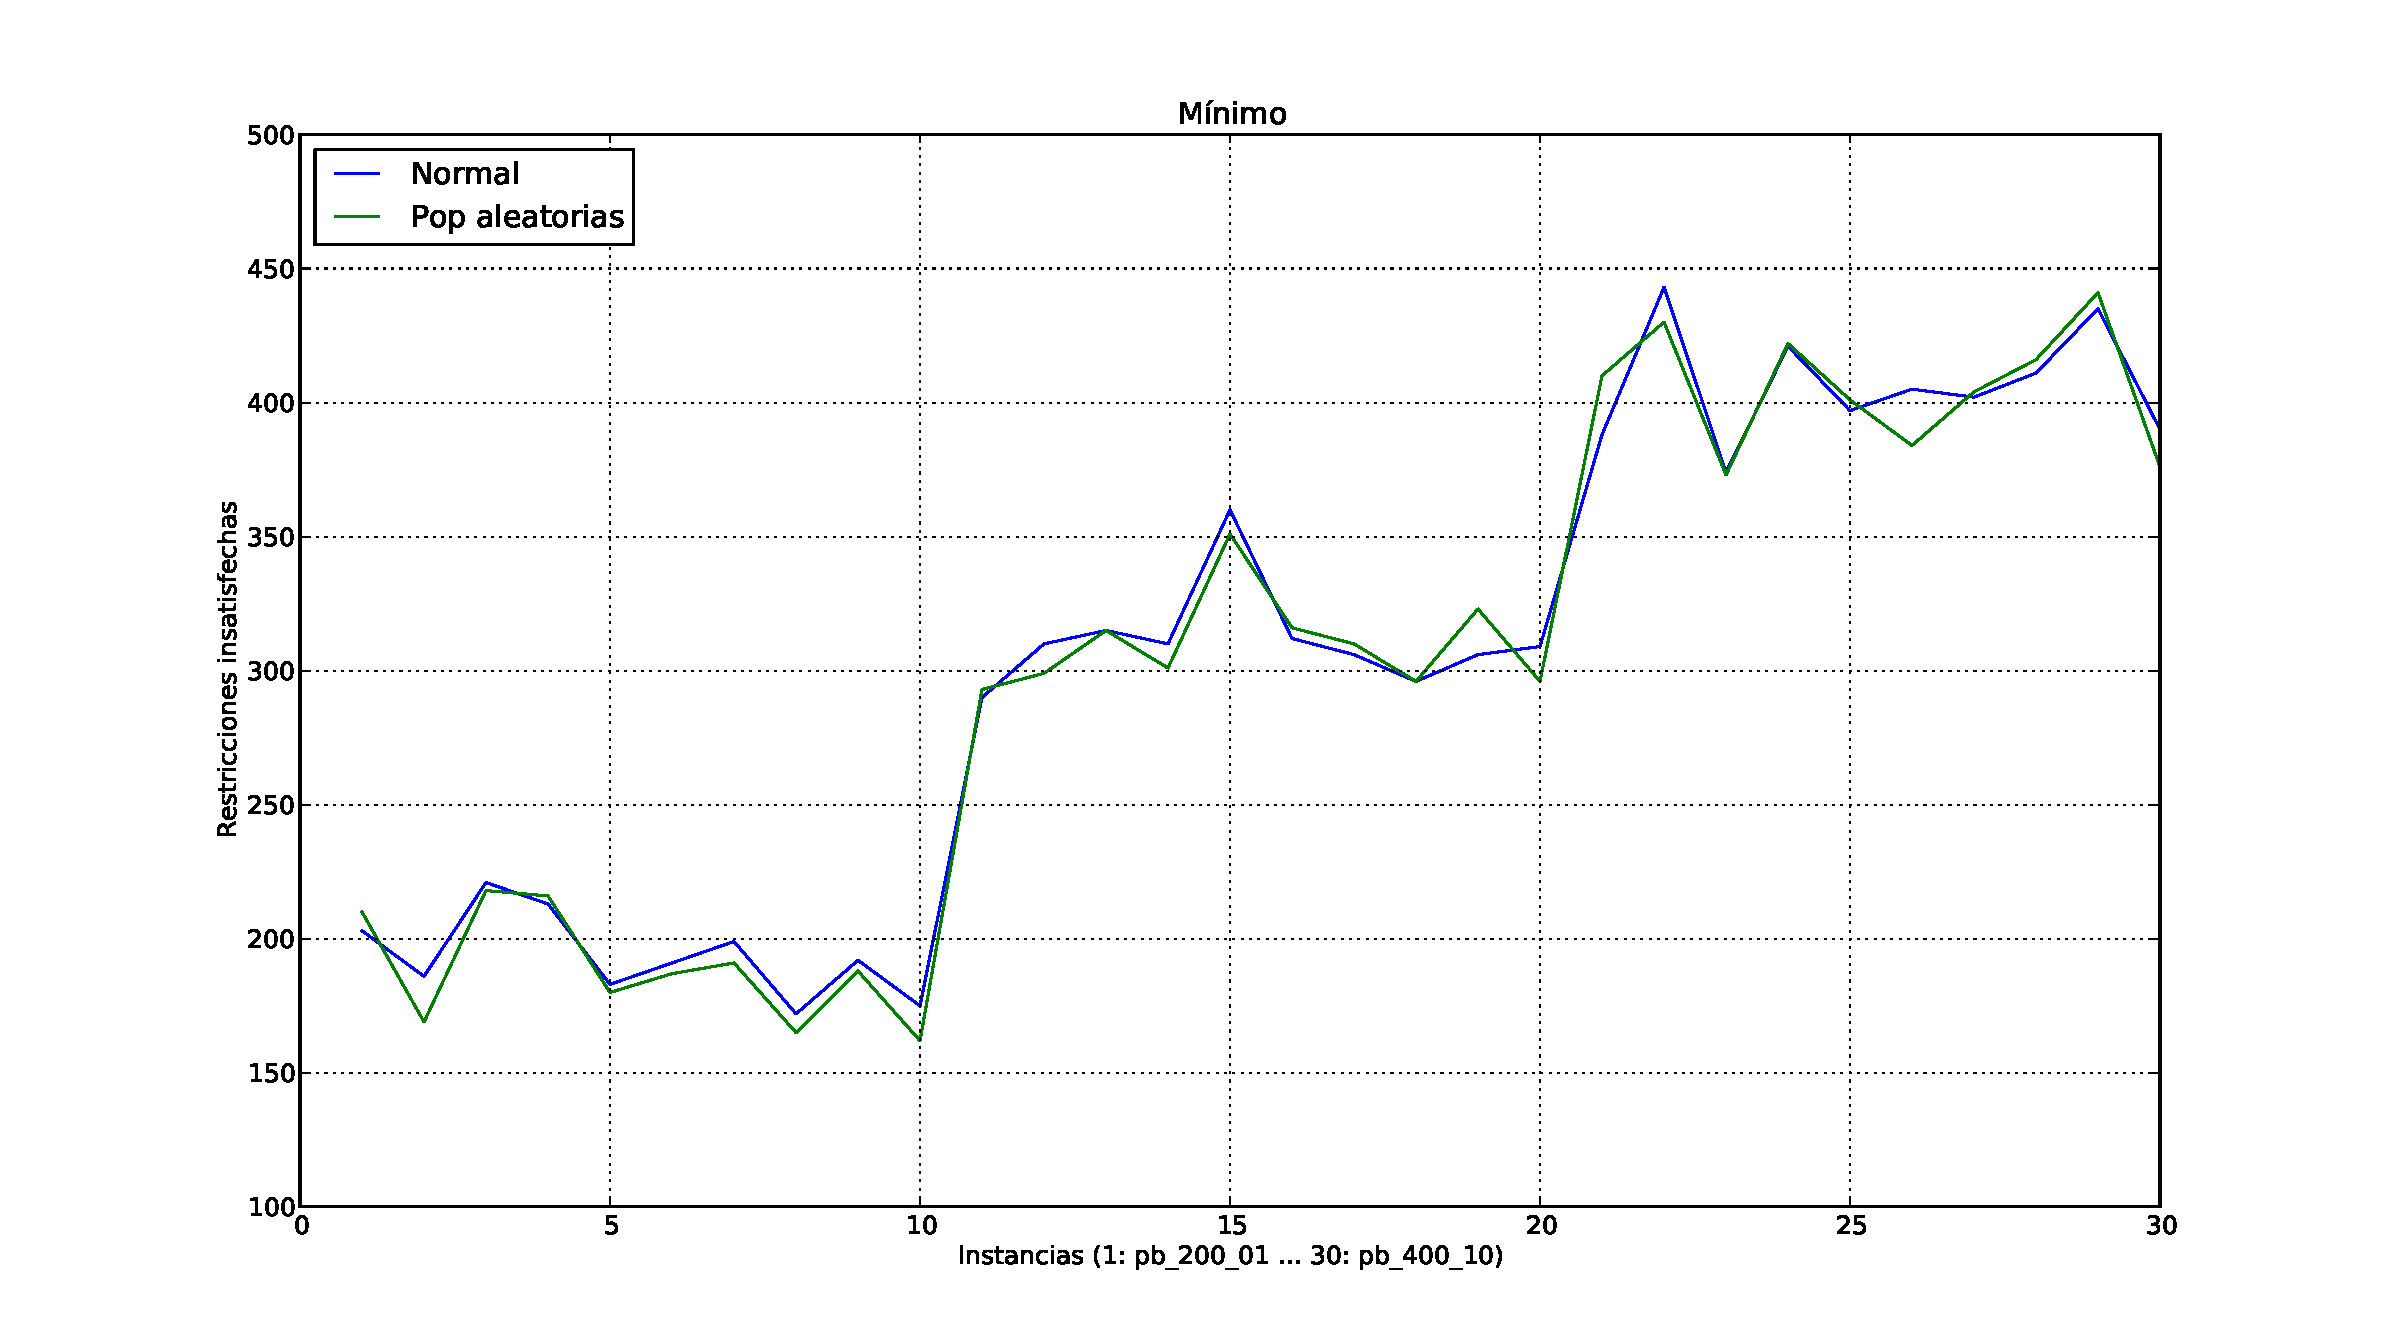
\includegraphics[width=0.8\textwidth]{img/min-1.pdf}
\end{center}
\caption{Valores mínimos para cada modificación}
\label{fig:min-1}
\end{figure}

\begin{figure}[h!]
\begin{center}
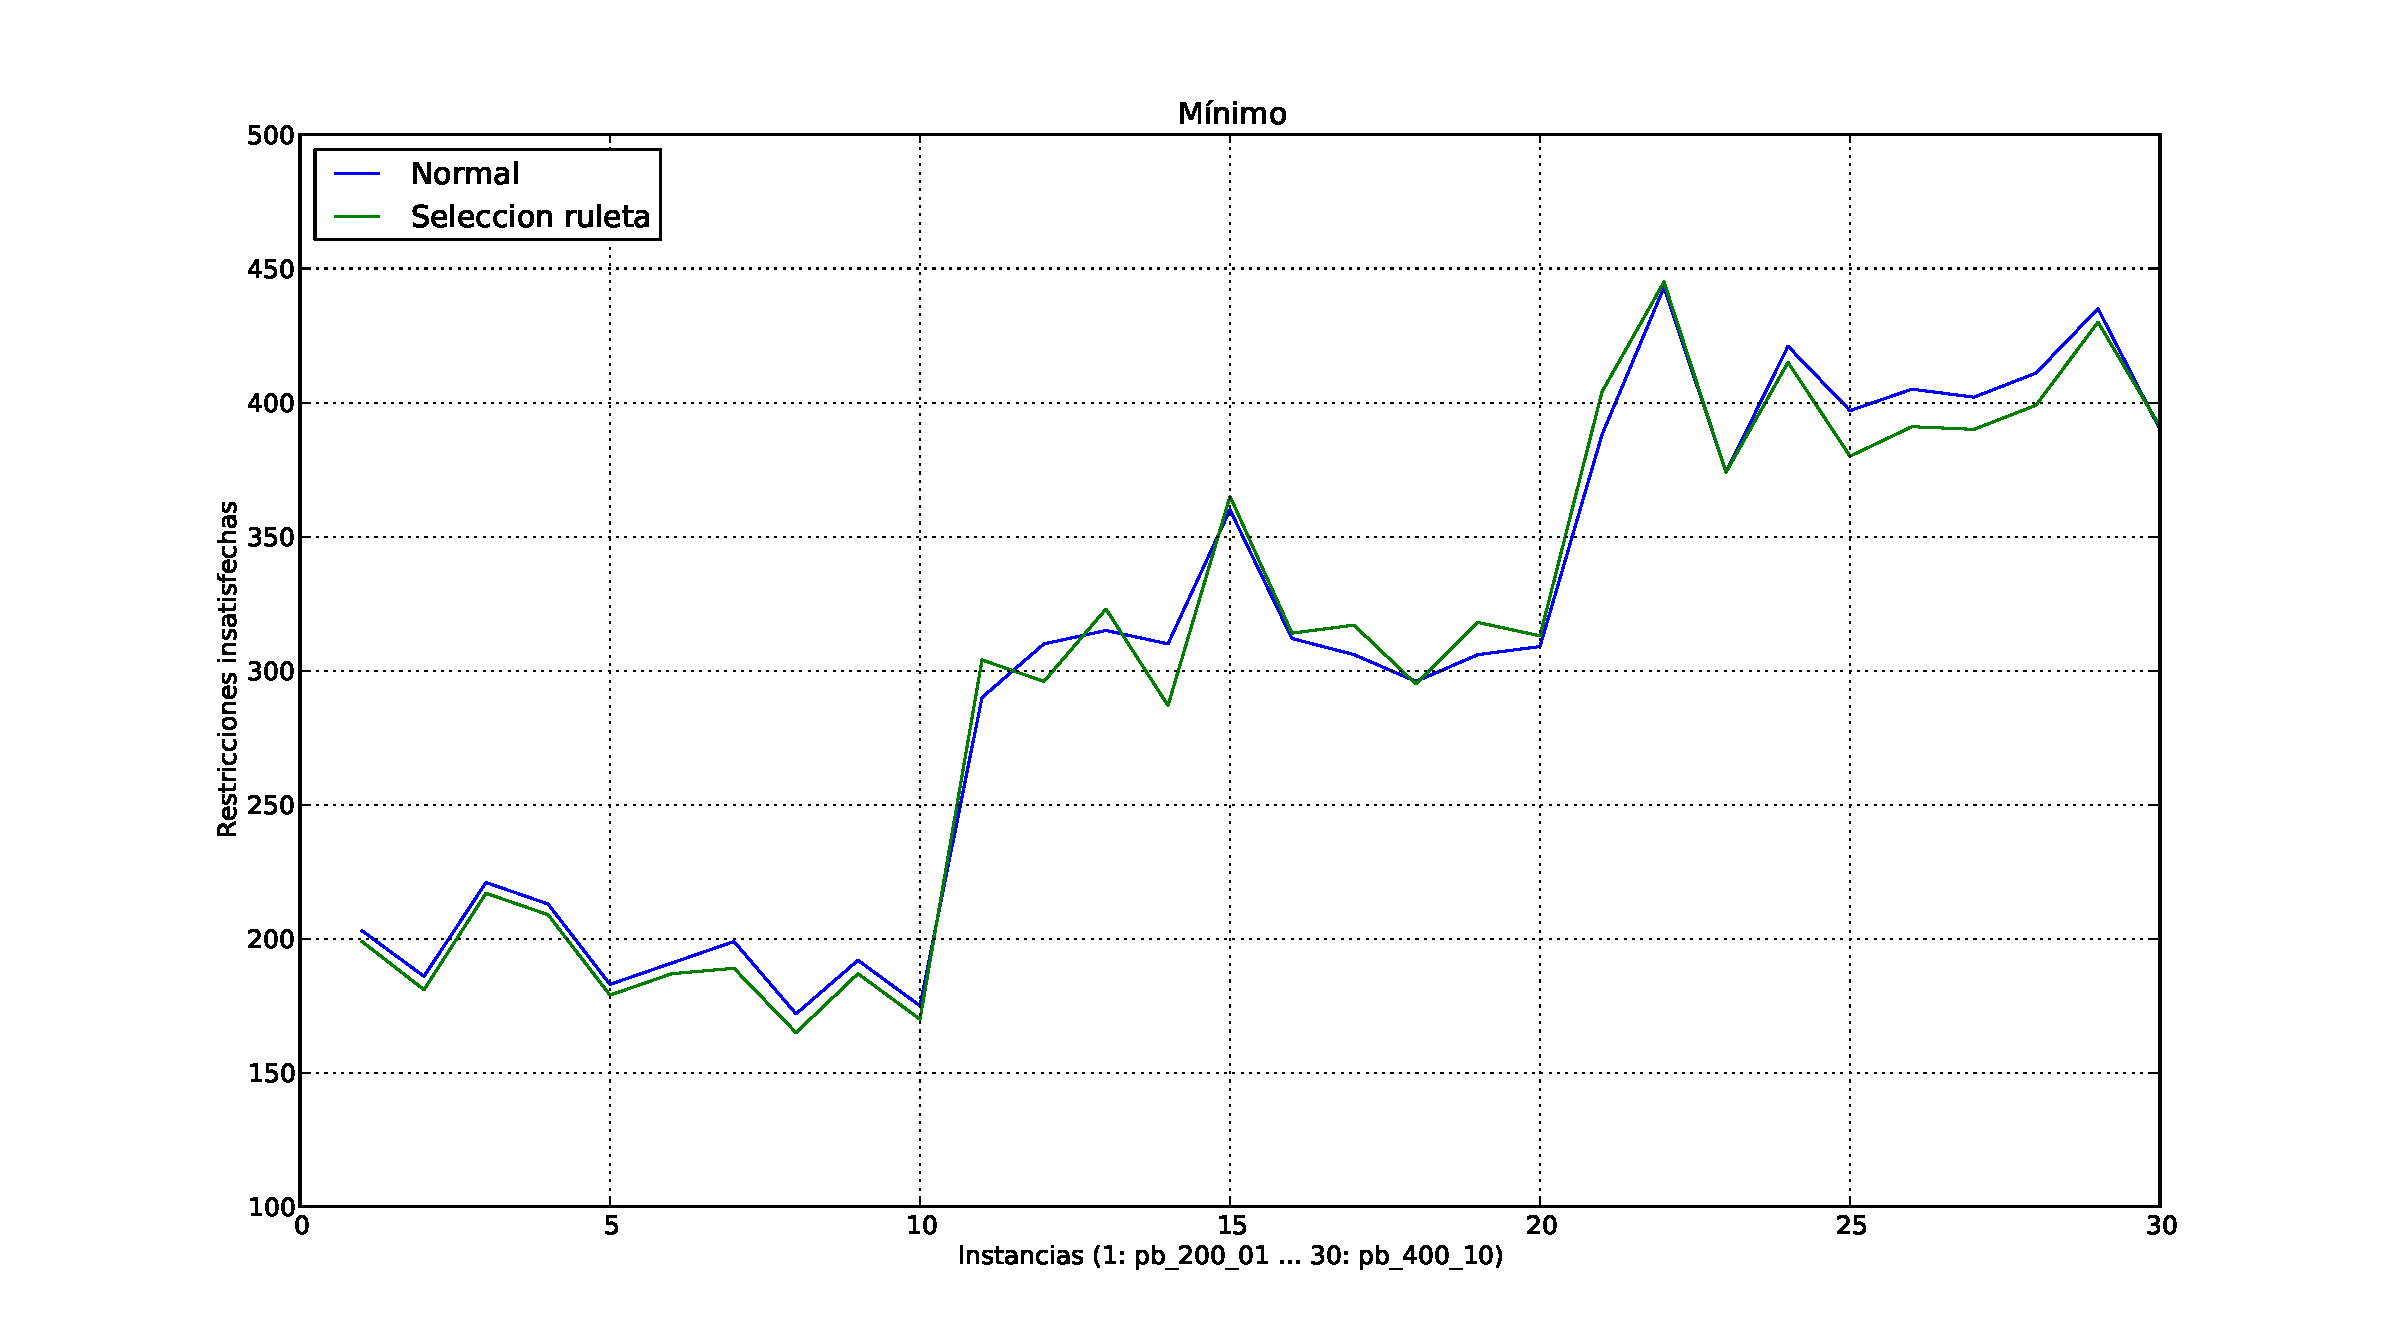
\includegraphics[width=0.8\textwidth]{img/min-2.pdf}
\end{center}
\caption{Valores mínimos para cada modificación}
\label{fig:min-2}
\end{figure}

\begin{figure}[h!]
\begin{center}
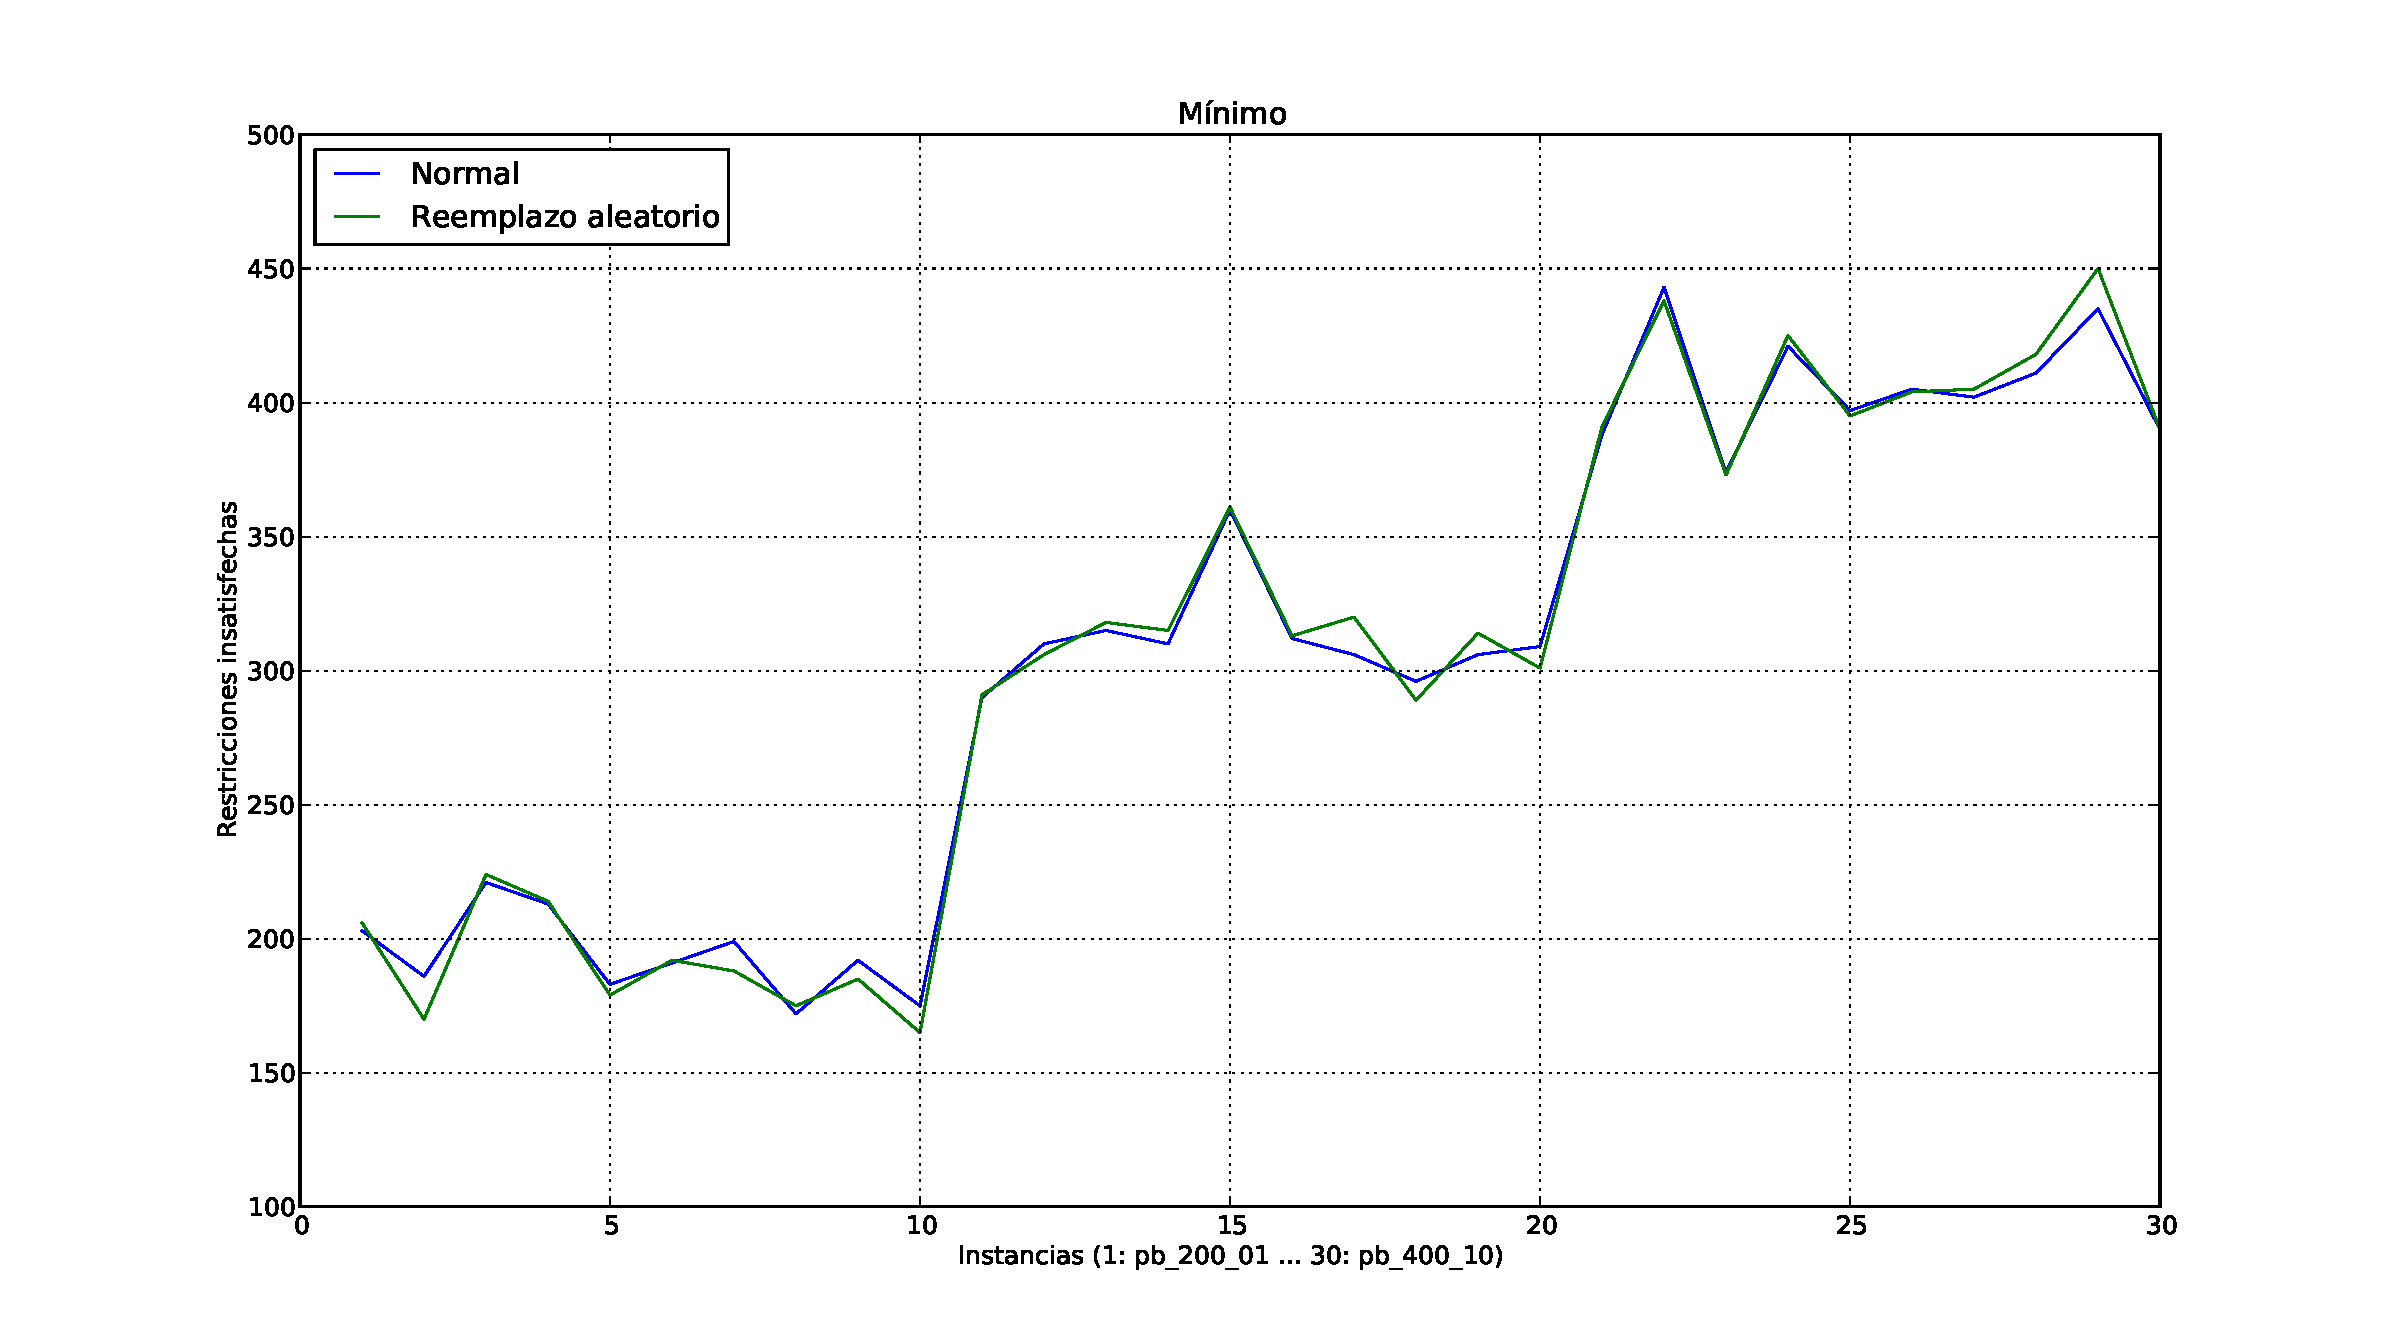
\includegraphics[width=0.8\textwidth]{img/min-3.pdf}
\end{center}
\caption{Valores mínimos para cada modificación}
\label{fig:min-3}
\end{figure}

\begin{figure}[h!]
\begin{center}
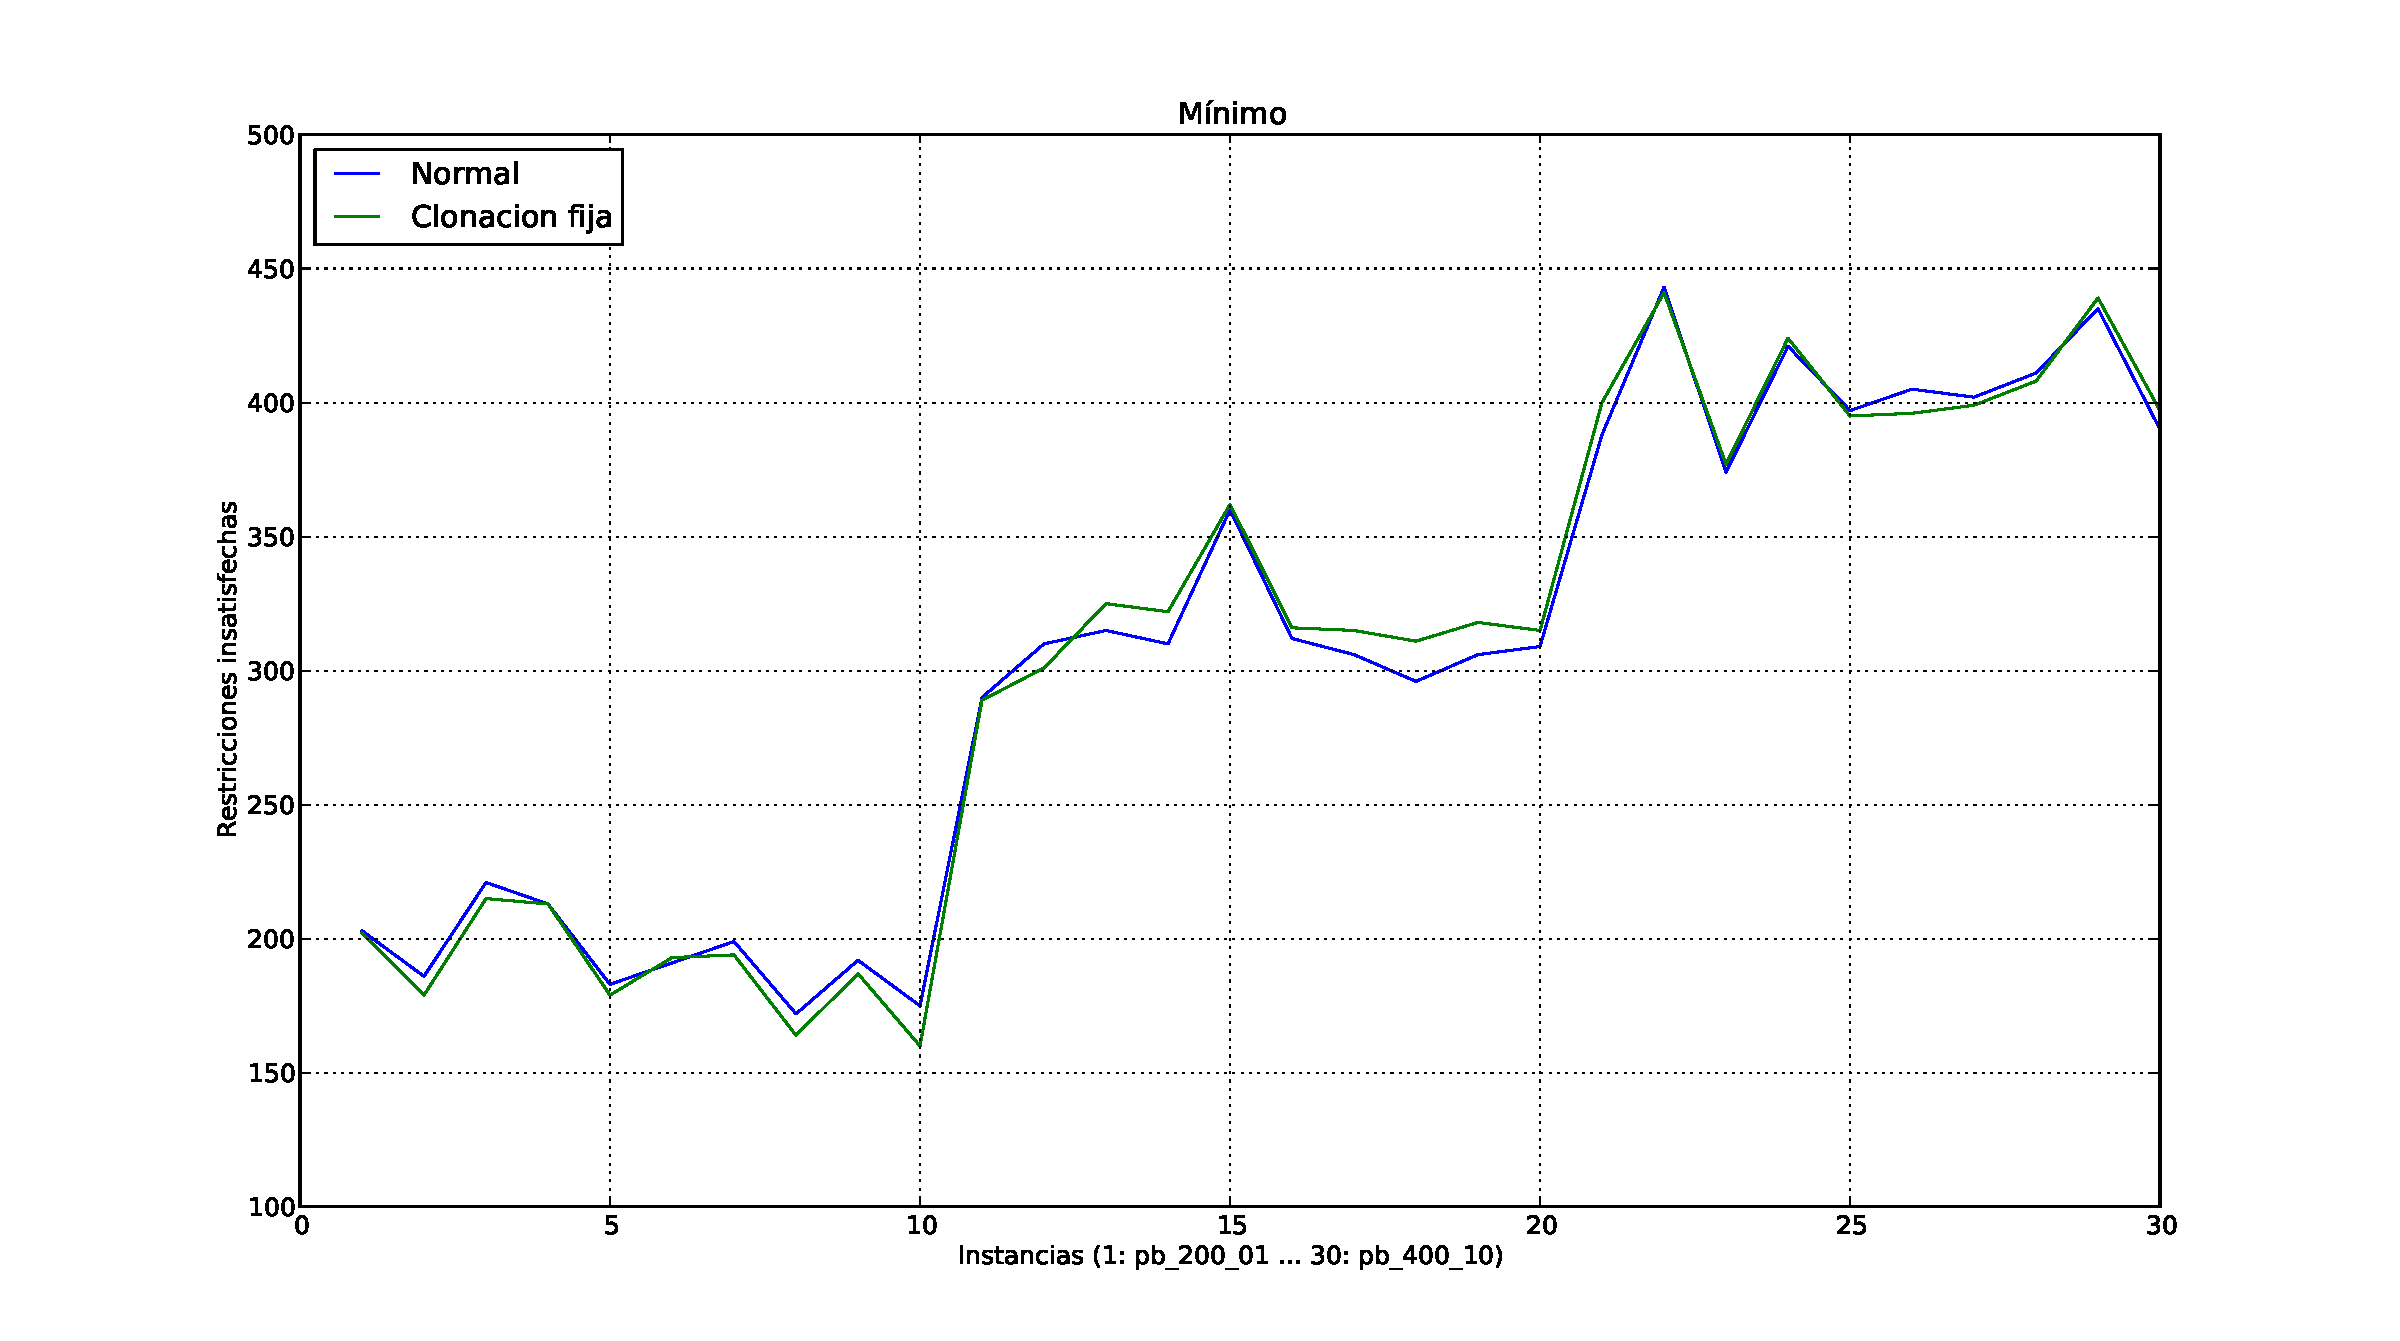
\includegraphics[width=0.8\textwidth]{img/min-4.pdf}
\end{center}
\caption{Valores mínimos para cada modificación}
\label{fig:min-4}
\end{figure}


\newpage
\subsection{Tiempo de ejecución}

\begin{figure}[h!]
\begin{center}
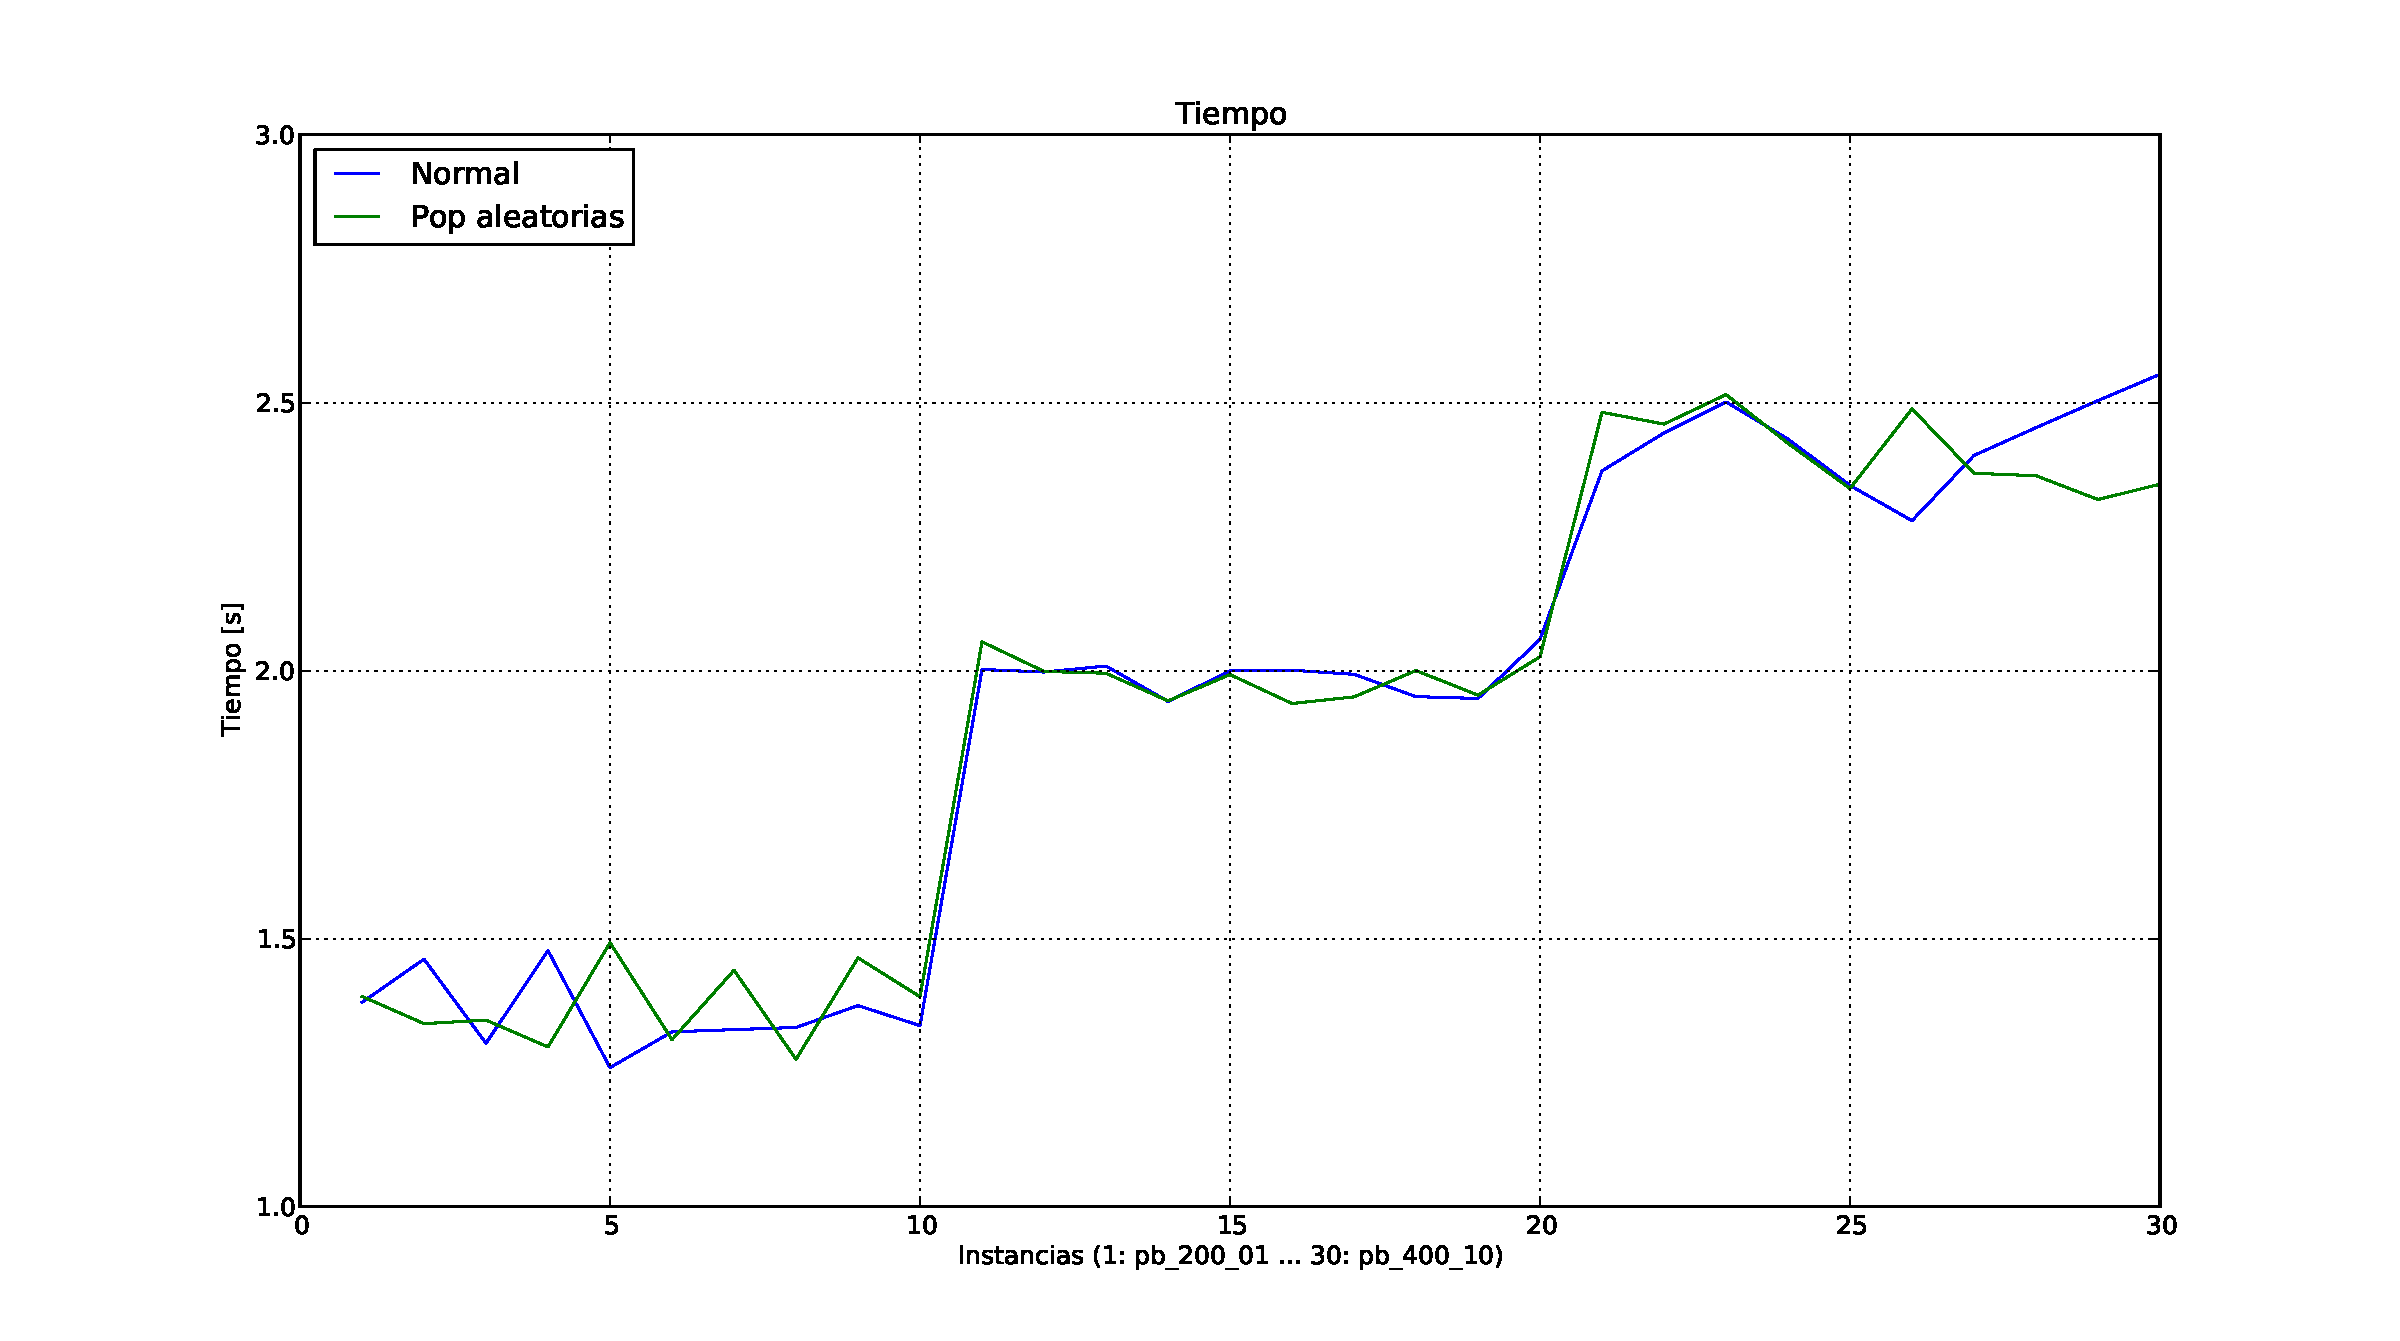
\includegraphics[width=0.95\textwidth]{img/t-1.pdf}
\end{center}
\caption{Tiempo de ejecución para las modificaciones en cada instancia}
\label{fig:t-1}
\end{figure}

\begin{figure}[h!]
\begin{center}
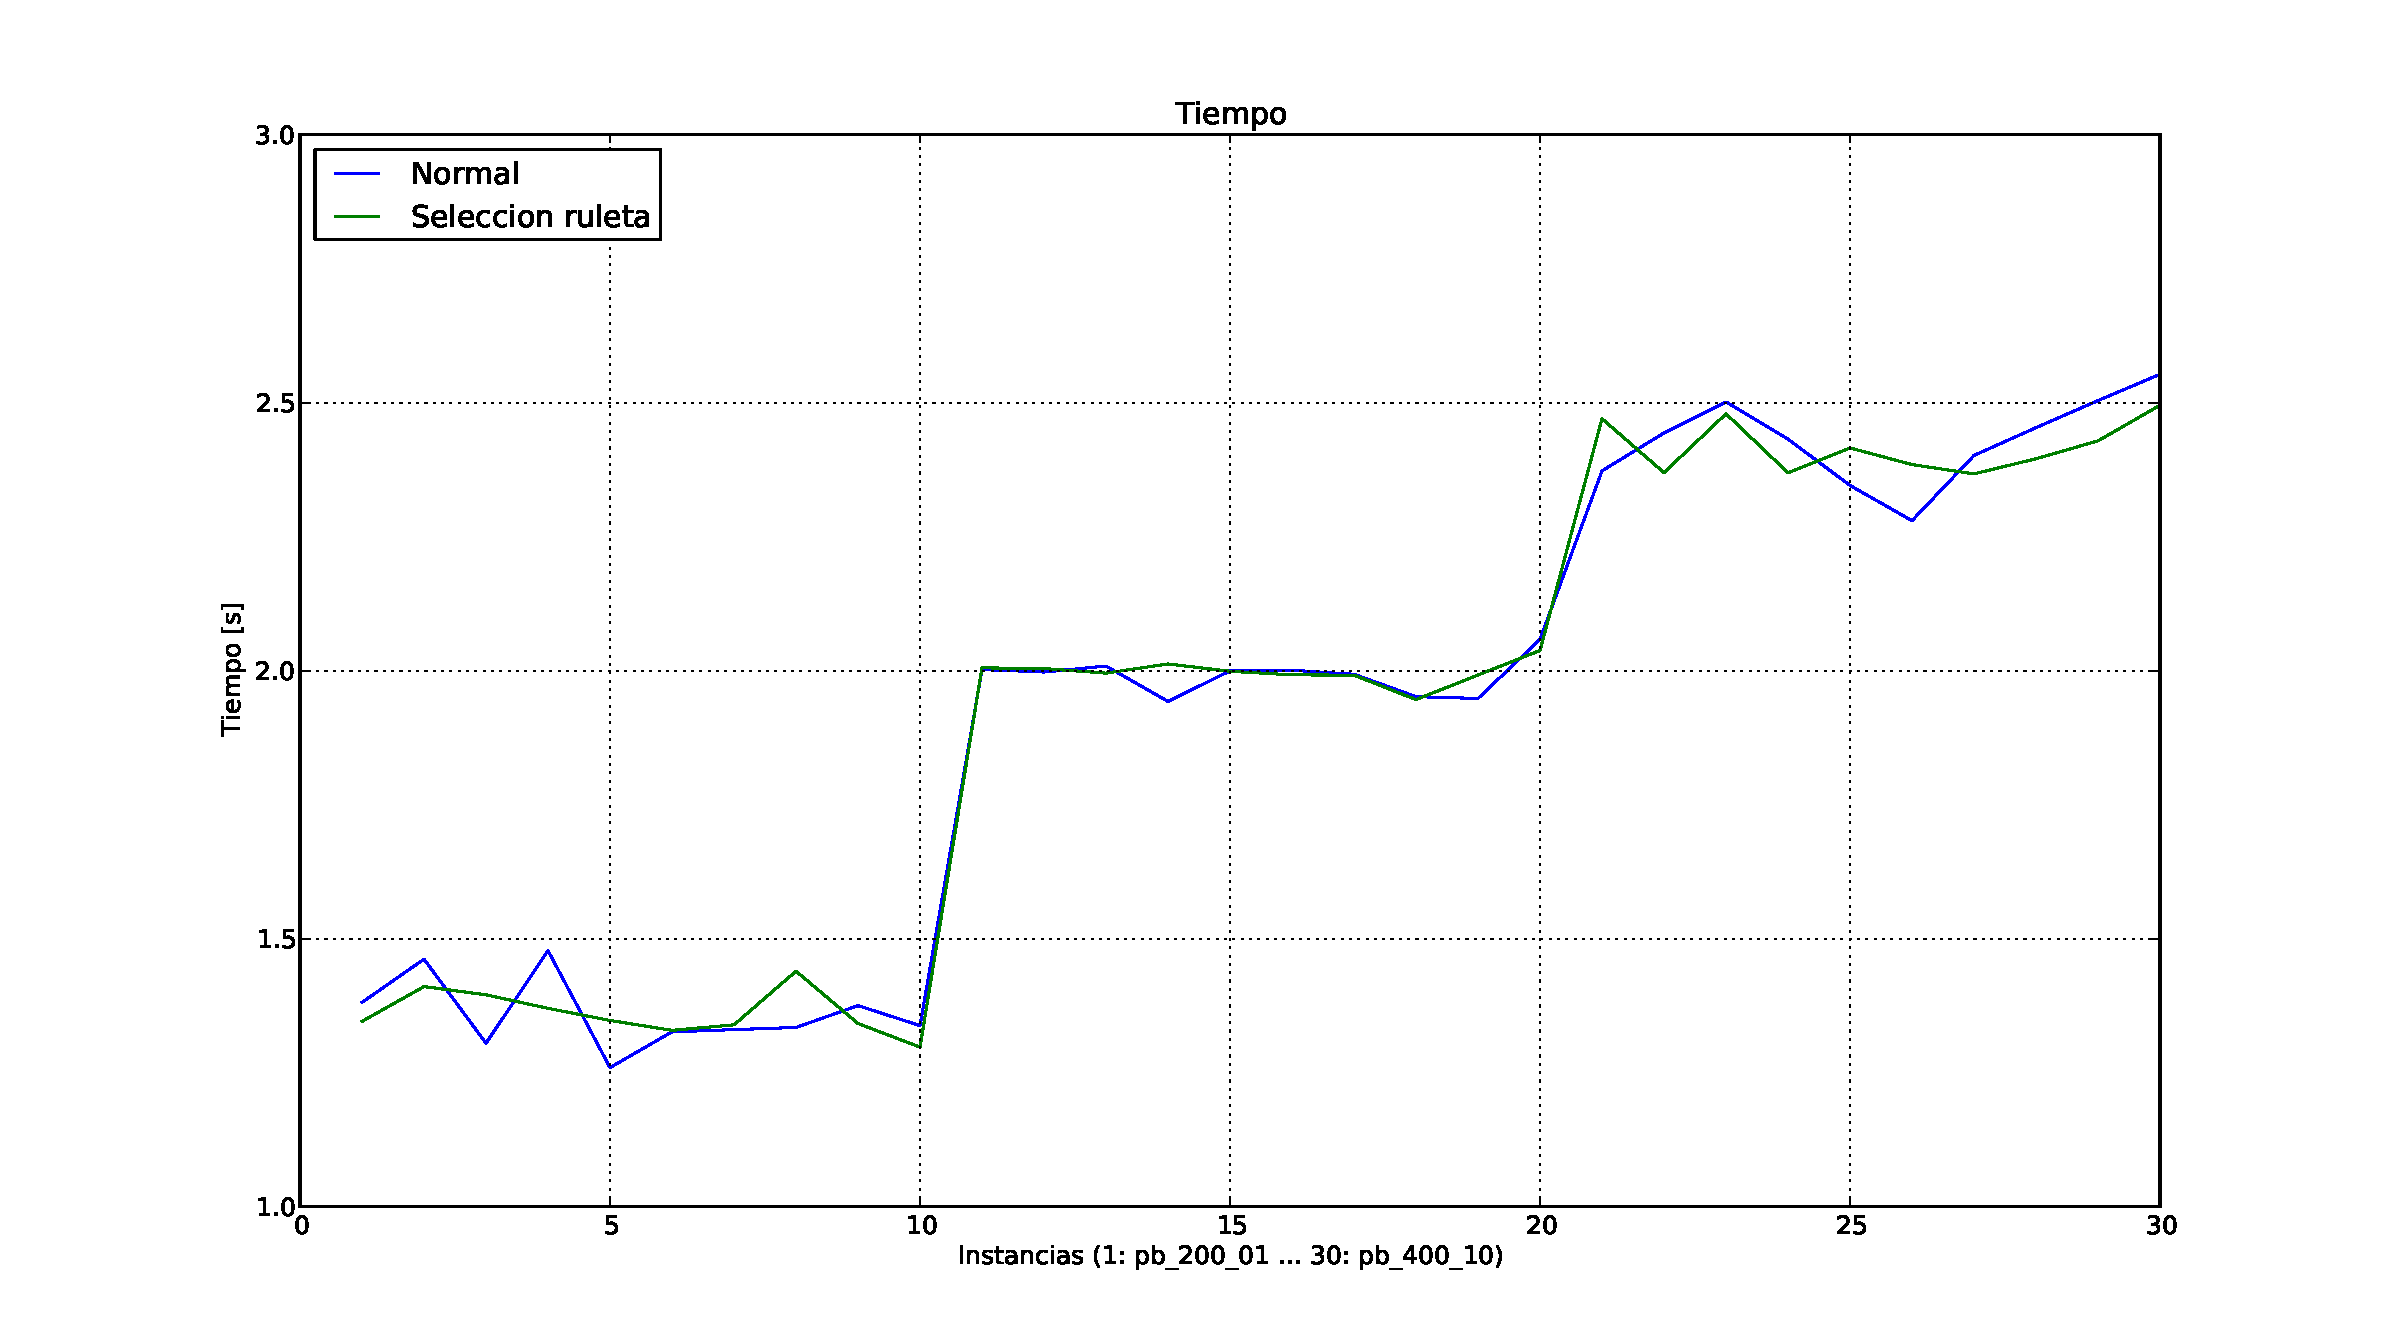
\includegraphics[width=0.95\textwidth]{img/t-2.pdf}
\end{center}
\caption{Tiempo de ejecución para las modificaciones en cada instancia}
\label{fig:t-2}
\end{figure}

\begin{figure}[h!]
\begin{center}
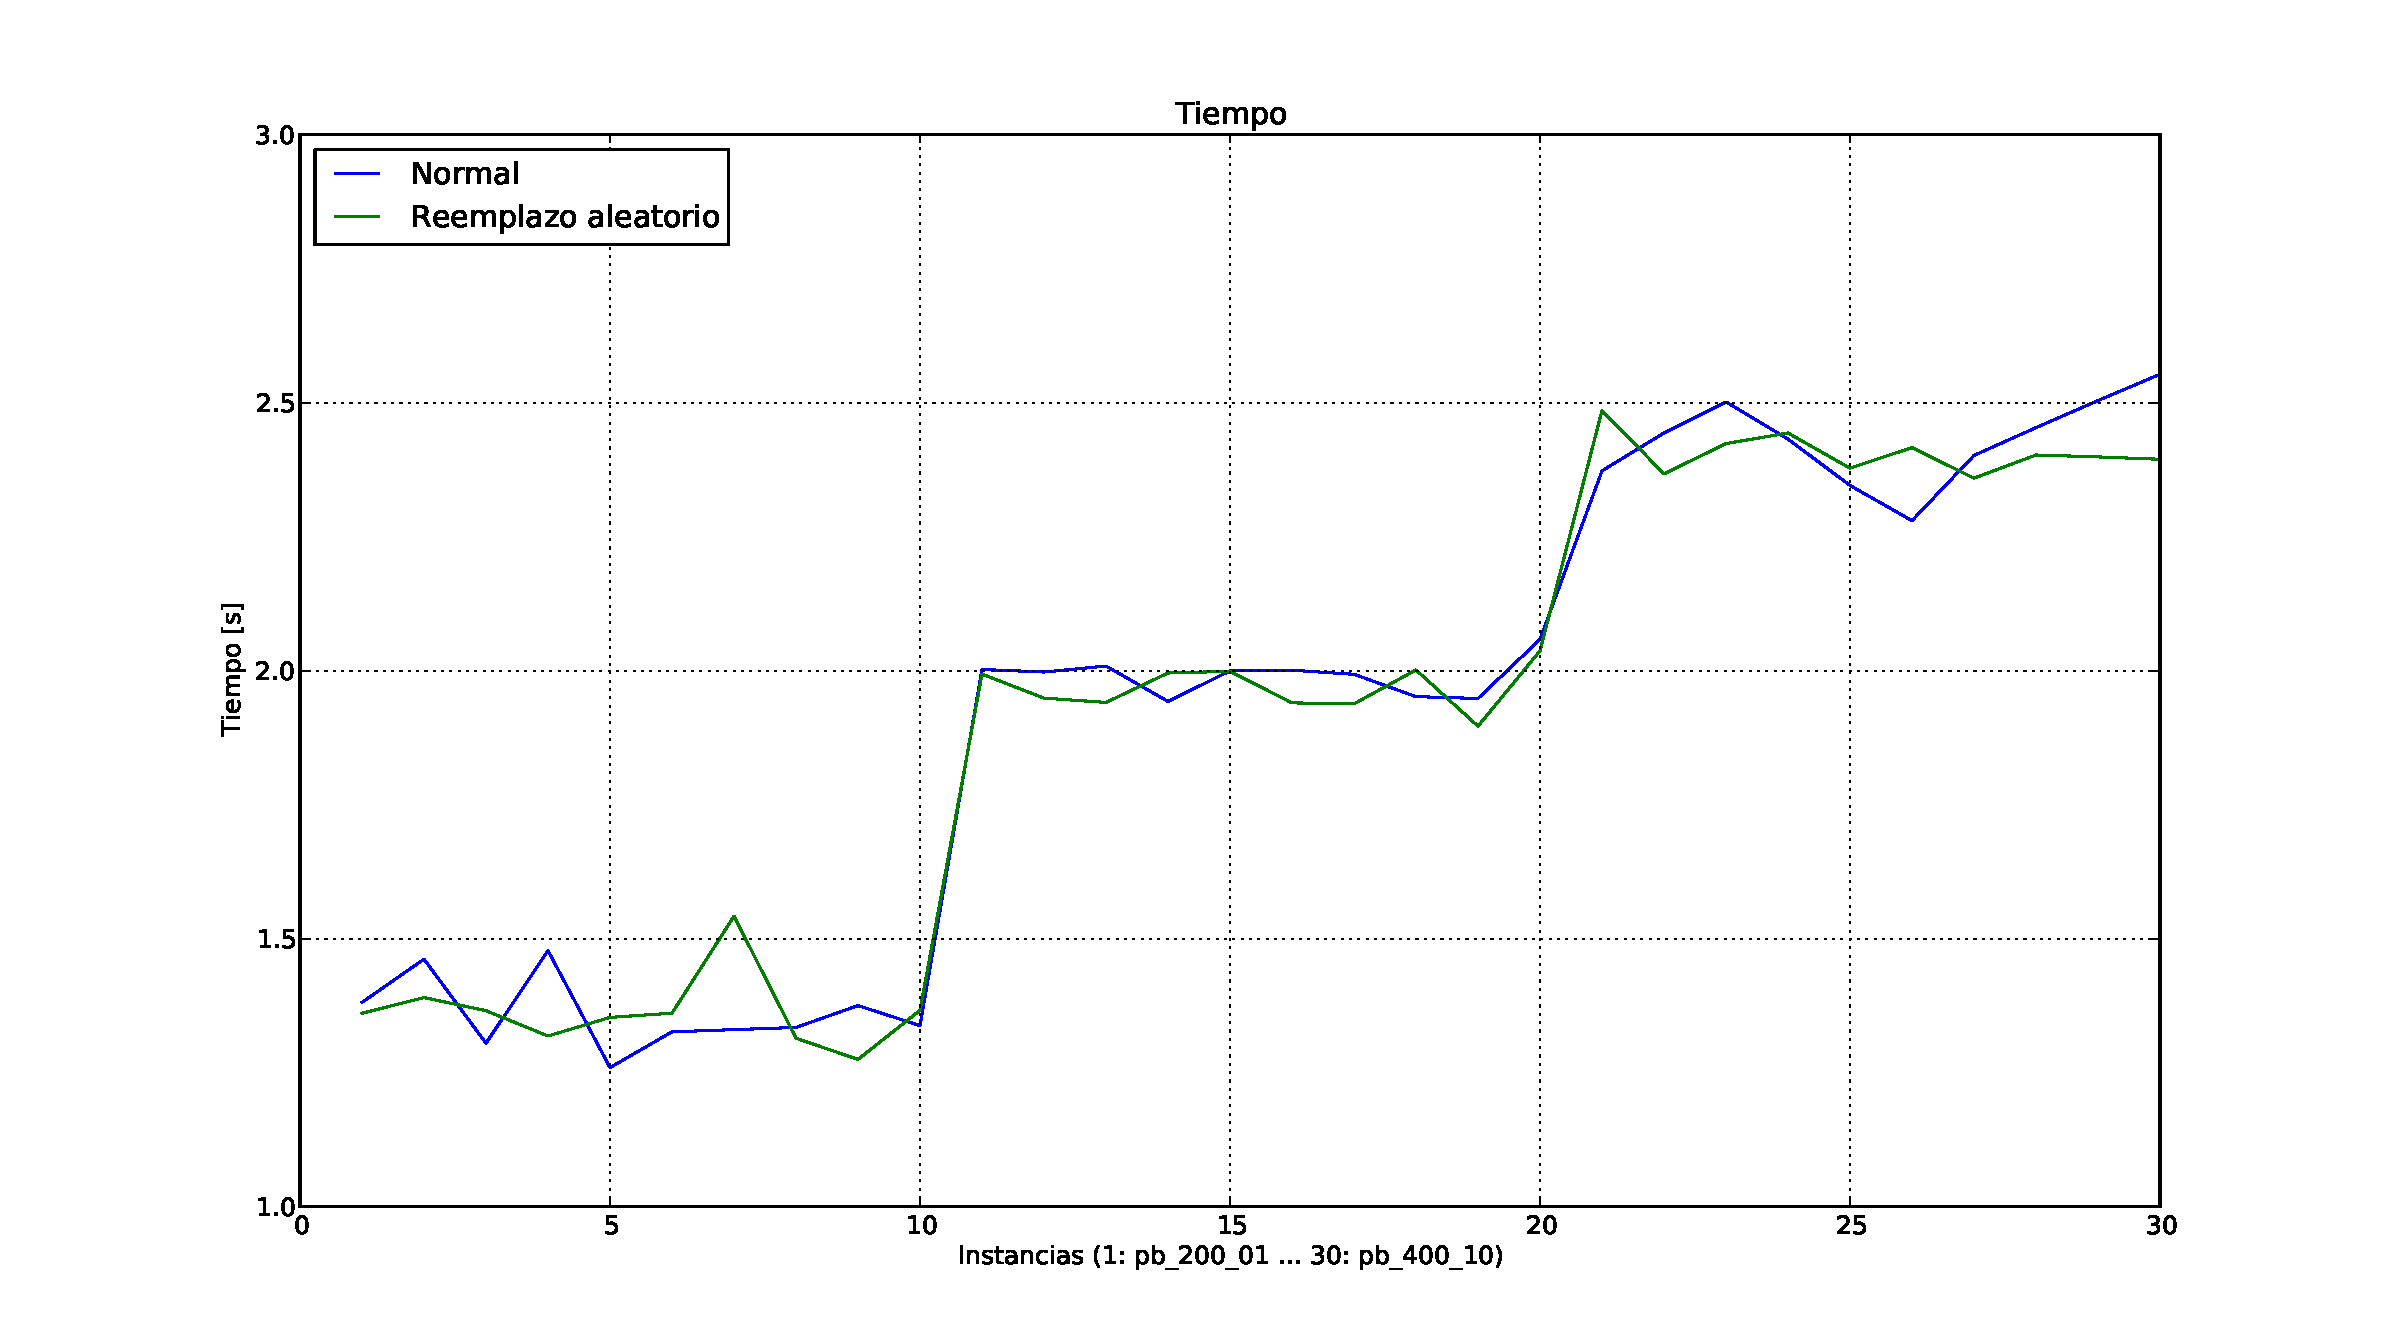
\includegraphics[width=0.95\textwidth]{img/t-3.pdf}
\end{center}
\caption{Tiempo de ejecución para las modificaciones en cada instancia}
\label{fig:t-3}
\end{figure}

\begin{figure}[h!]
\begin{center}
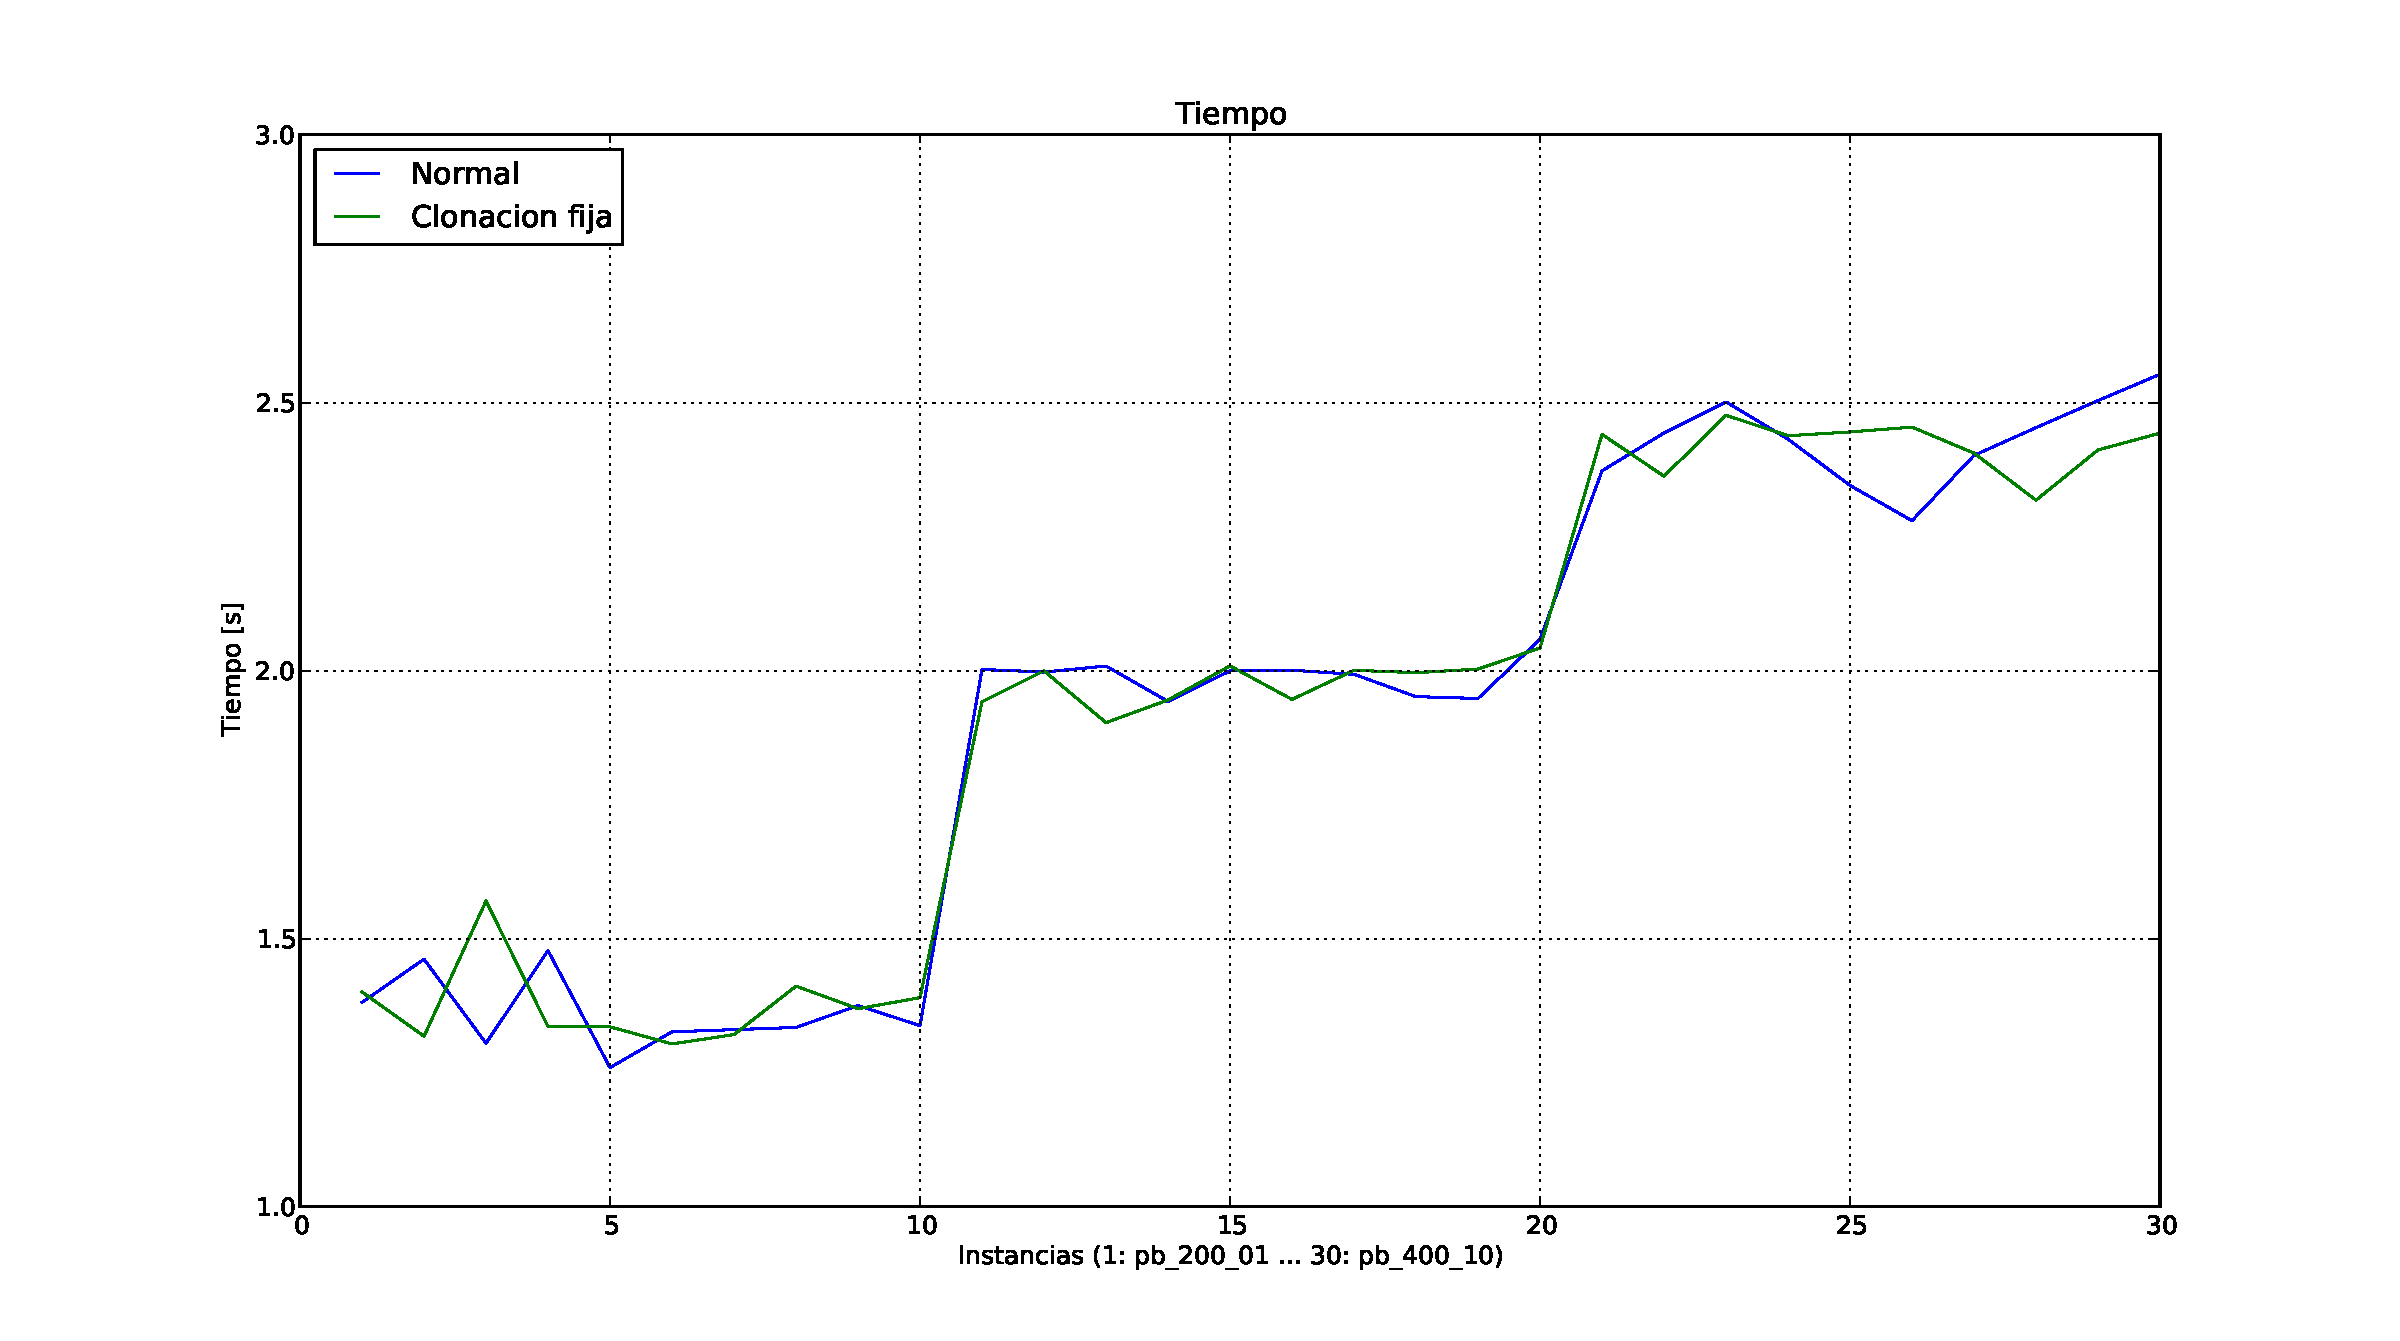
\includegraphics[width=0.95\textwidth]{img/t-4.pdf}
\end{center}
\caption{Tiempo de ejecución para las modificaciones en cada instancia}
\label{fig:t-4}
\end{figure}
